\ifx\wholebook\relax \else

\documentclass[b5paper]{article}
\usepackage[nomarginpar
  %, margin=.5in
]{geometry}

\addtolength{\oddsidemargin}{-0.05in}
\addtolength{\evensidemargin}{-0.05in}
\addtolength{\textwidth}{0.1in}
\usepackage[en]{../../../prelude}

\setcounter{page}{1}

\begin{document}

\title{B-Tree}

\author{Xinyu LIU
\thanks{{\bfseries Xinyu LIU} \newline
  Email: liuxinyu95@gmail.com \newline}
  }

\maketitle
\fi

\markboth{B-Tree}{Elementary Algorithms}

\ifx\wholebook\relax
\chapter{B-Tree}
\numberwithin{Exercise}{chapter}
\fi

\section{Introduction}
\index{B-tree}
\label{introduction}

The integer prefix tree in previous chapter gives a way to encode the information in the edge of the binary tree. Another way to extend the binary search tree is to increase the sub-trees from 2 to $k$. B-tree is such a data structure, that can be considered as a generic form of $k$-ary search tree. It is also developed to be self-balanced\cite{wiki-b-tree}. B-tree is widely used in computer file system (some are based on B+ tree, an extension of B-tree) and database system. \Cref{fig:btree-example} gives an example B-tree, we can find the difference and similarity between B-tree and binary search tree.

\begin{figure}[htbp]
  \centering
  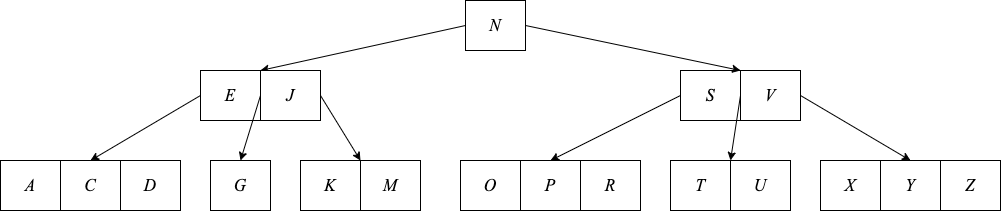
\includegraphics[scale=0.33]{img/btree-del-before}
  \caption{A B-Tree}
  \label{fig:btree-example}
\end{figure}

A binary search tree is either empty or contains a key $k$ and two sub-trees $l$ and $r$. Every key in $l$ is less than $k$, while $k$ is less than every key in $r$:

\be
\forall\ x \in l, y \in r \Rightarrow x < k < y
\ee

Extend to multiple keys and sub-trees, we obtain the B-tree. A B-tree is either empty or contains $n$ keys and $n + 1$ sub-trees, each sub-tree is also a B-Tree. We denote these keys and sub-trees as $k_1, k_2, ..., k_n$ and $t_1, t_2, ..., t_n, t_{n+1}$, as shown in \cref{fig:btree-node}.

\begin{figure}[htbp]
  \centering
  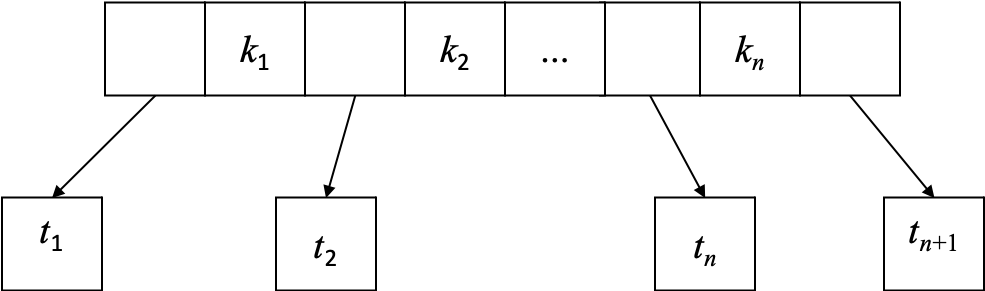
\includegraphics[scale=0.5]{img/btree-node}
  \caption{A B-Tree node}
  \label{fig:btree-node}
\end{figure}

For every node, the keys and sub-trees satisfy the following rules:

\begin{itemize}
\item Keys are in ascending order: $k_1 < k_2 < ... < k_n$;
\item For every key $k_i$, all keys in sub-tree $t_i$ are less than it, while $k_i$ is less than every key in sub-tree $t_{i+1}$:
\end{itemize}

\begin{equation}
\forall\ x_i \in t_i, i=0, 1, ..., n\ \Rightarrow x_1 < k_1 < x_2 < k_2 < ... < x_n < k_n < x_{n+1}
\label{eq:btree-order}
\end{equation}

Leaf node has no sub-tree. There can be optional values bound to the keys in B-tree node. We skip the values for simplicity. Let the type of keys be $K$, the type of the B-tree is $BTree\ K$, or denoted as \texttt{BTree<K>}. On top of it, we also need define a set of self-balance rules:

\begin{enumerate}
\item All leaves have the same depth;
\item Let $d$ be the {\em minimum degree} number of a B-tree, such that each node:
  \begin{itemize}
  \item has at most $2d - 1$ keys;
  \item has at least $d - 1$ keys, except for the root;
  \end{itemize}
\end{enumerate}

In summary:

\be
  d - 1 \leq |keys(t)|  \leq 2d - 1
\ee

We next prove that a B-tree satisfying these rules is always balanced.

\begin{proof}
Consider a B-tree of $n$ keys. The minimum degree $d \geq 2$. Let the height be $h$. All the nodes have at least $d - 1$ keys except for the root. The root contains at least 1 key. There are at least 2 nodes at depth 1, at least $2d$ nodes at depth 2, at least $2d^2$ nodes at depth 3, ..., at least $2d^{h-1}$ nodes at depth $h$. Multiply all nodes with $d-1$ except for the root, the total number of keys satisfies the following:

\be
\begin{array}{rl}
n & \geq 1 + (d - 1)(2 + 2d + 2d^2 + ... + 2d^{h-1}) \\
  & = 1 + 2(d - 1) \displaystyle \sum_{k=0}^{h-1} d^k \\
  & = 1 + 2(d - 1) \displaystyle \frac{d^h-1}{d-1} \\
  & = 2d^h - 1
\end{array}
\ee

It limits the tree height with logarithm of the number of keys.

\be
h \leq \log_d \frac{n+1}{2}
\ee

\end{proof}

Hence B-tree is balanced. The simplest B-tree is called 2-3-4 tree, where $d = 2$. Every node except for the root contains 2, 3, or 4 sub-trees. Essentially, a red-black tree can be mapped to a 2-3-4 tree. For a none empty B-tree of degree $d$, we denote it as $(d, (ks, ts))$, where $ks$ are the keys, $ts$ are the sub-trees. Below example program defines the B-tree.

\lstset{frame = single}
\begin{Haskell}
data BTree a = BTree [a] [BTree a]
\end{Haskell}

The empty node is in the form of $(\nil, \nil)$ or \texttt{BTree [] []}. Instead of storing $d$ in every node, we pass it together with B-tree $t$ as a pair $(d, t)$.

\section{Insert}
\label{btree-insertion} \index{B-tree!insert}

The idea is similar to the binary search tree. While we need deal with multiple keys and sub-trees. When insert key $x$ to B-tree $t$, starting from the root, we examine the keys in the node to locate a position\footnote{In fact, it is sufficient to only support less-than and equality. See \cref{ex:btree-leq}.} where all keys on the left are less than $x$, while the rest keys on the right are greater than $x$. If the node is a leaf, and it is not full ($|keys(t)| < 2d - 1$), we insert $x$ at this position. Otherwise, this position points to a sub-tree $t'$, we recursively insert $x$ to $t'$.

\begin{figure}[htbp]
  \centering
  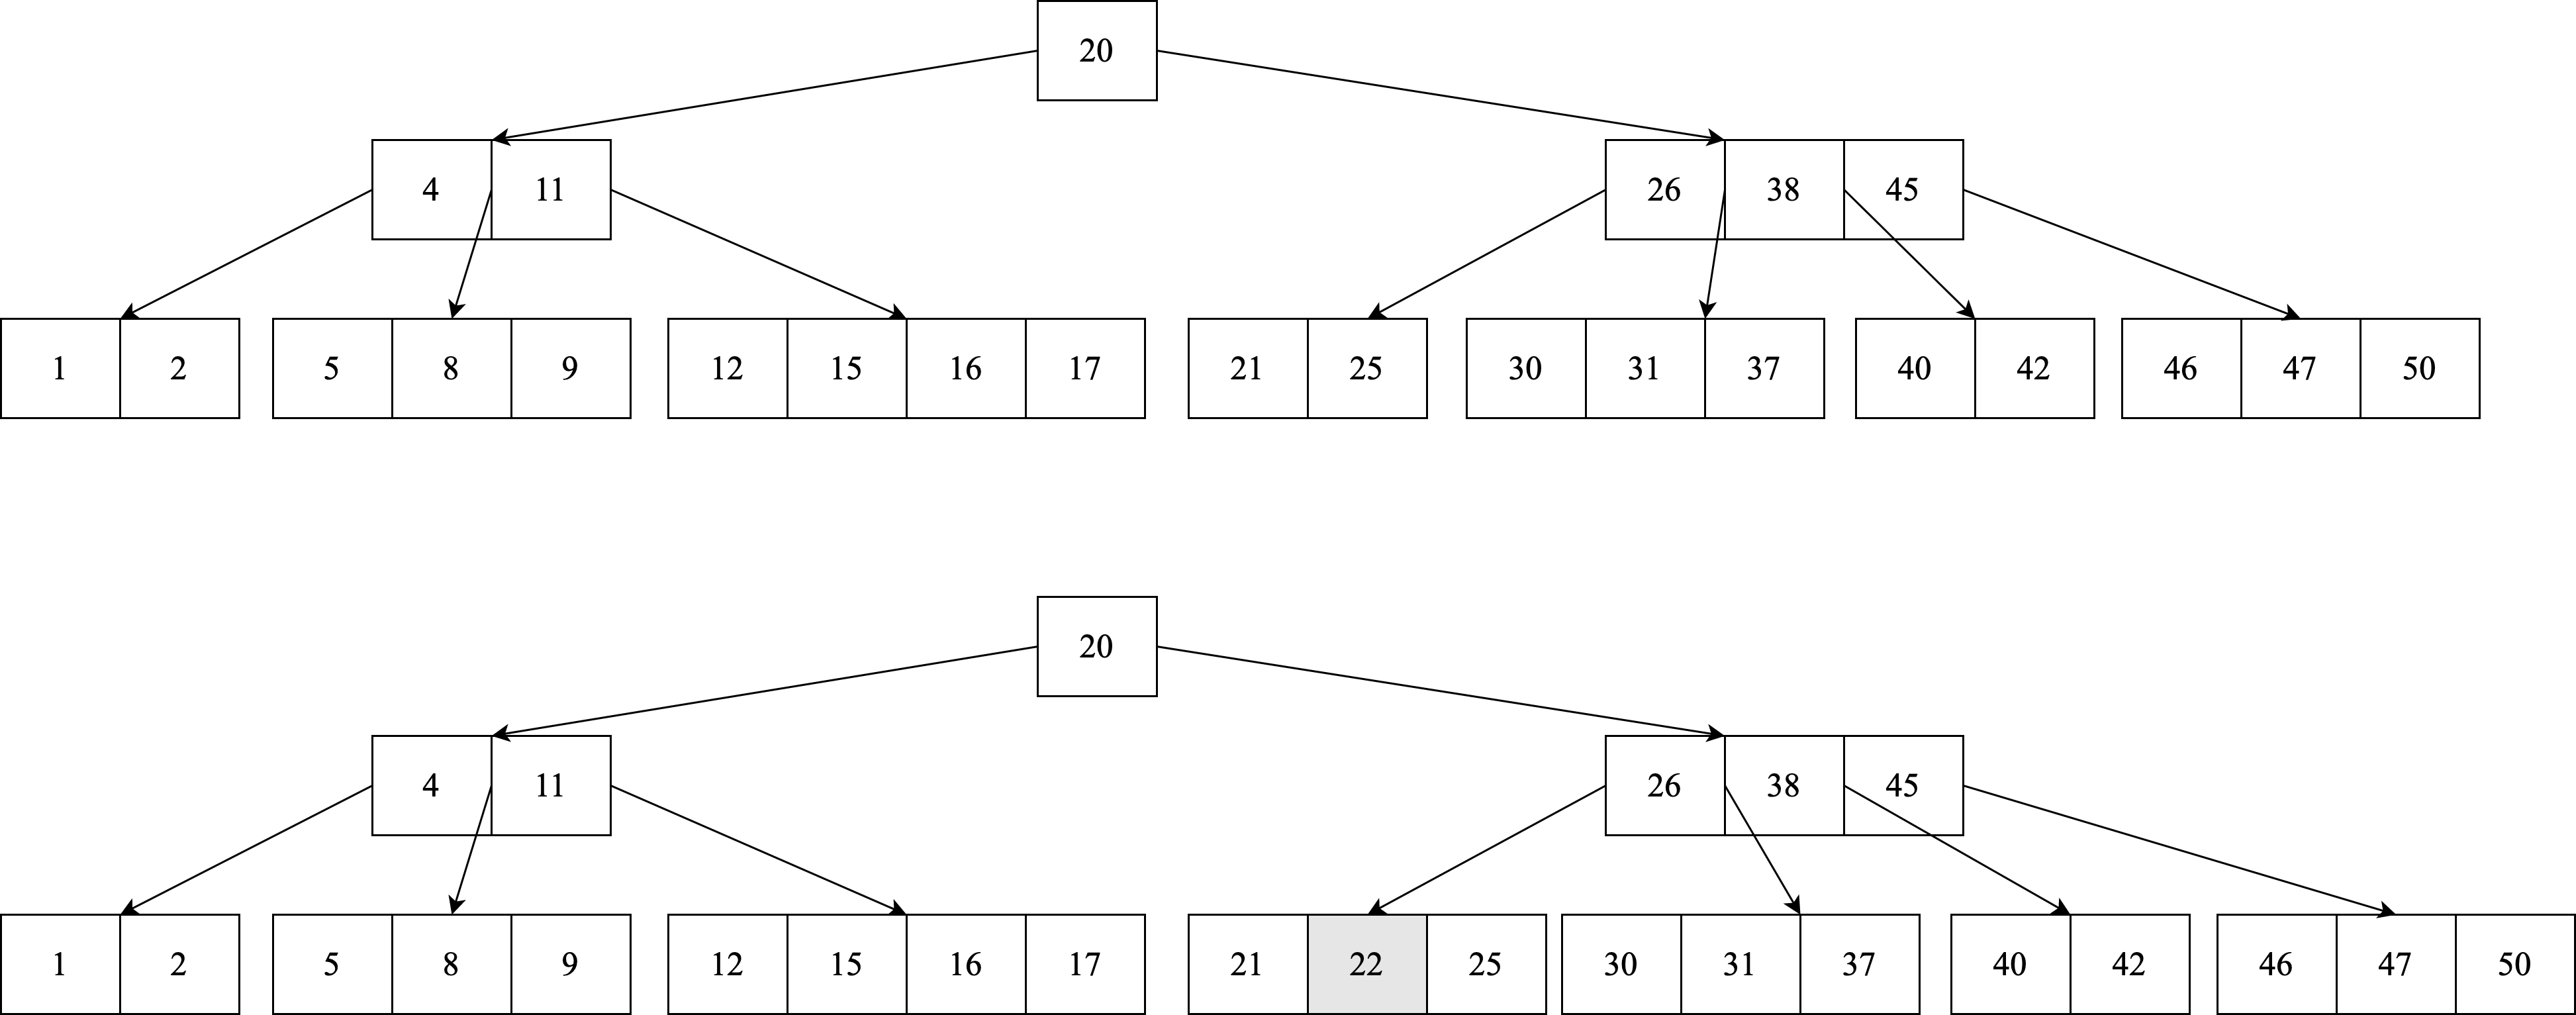
\includegraphics[scale=0.4]{img/btree-insert-example}
  \caption{Insert 22 to a 2-3-4 tree. $22 > 20$, go to the right sub-tree; next as $22 < 26$, go to the first sub-tree; finally, $21 < 22 < 25$, and the leaf is not full.}
  \label{fig:btree-insert-simple}
\end{figure}

As an example, consider the 2-3-4 tree in \cref{fig:btree-insert-simple}. when insert $x = 22$, because $20 < 22$, we next examine the sub-tree on the right, which contains 26, 38, 45. Since $22 < 26$, we next go to the first sub-tree containing 21 and 25. This is a leaf, and it is not full. Hence we insert 22 to this node.

However, if there are $2d - 1$ keys in the leaf, we will break the B-tree rules after insert $x$, as the node will be too 'full'. For the same B-tree in \cref{fig:btree-insert-simple}, we'll meet this issue when insert 18. There are two solutions: insert then split, and split before insert.

\subsection{Insert then split}

We can adopt the similar `insert then fix' method for the red-black tree. First, we insert the key to the proper ordering position without considering the B-tree balance rules. As the next step, if the new tree violates the balance rules, we perform a recursive bottom-up fixing by splitting the overly full node. We need define the function to test whether a given node satisfies the minimum degree constraint or not.


\be
\begin{cases}
full\ d\ (ks, ts) & = |ks| > 2d - 1 \\
low\  d\ (ks, ts) & = |ks| < d - 1 \\
\end{cases}
\ee

When the node contains too many keys and sub-trees, we define $split$ function to break it into 3 parts at a given position $m$ as shown in \cref{fig:node-split}:

\begin{figure}[htbp]
  \centering
  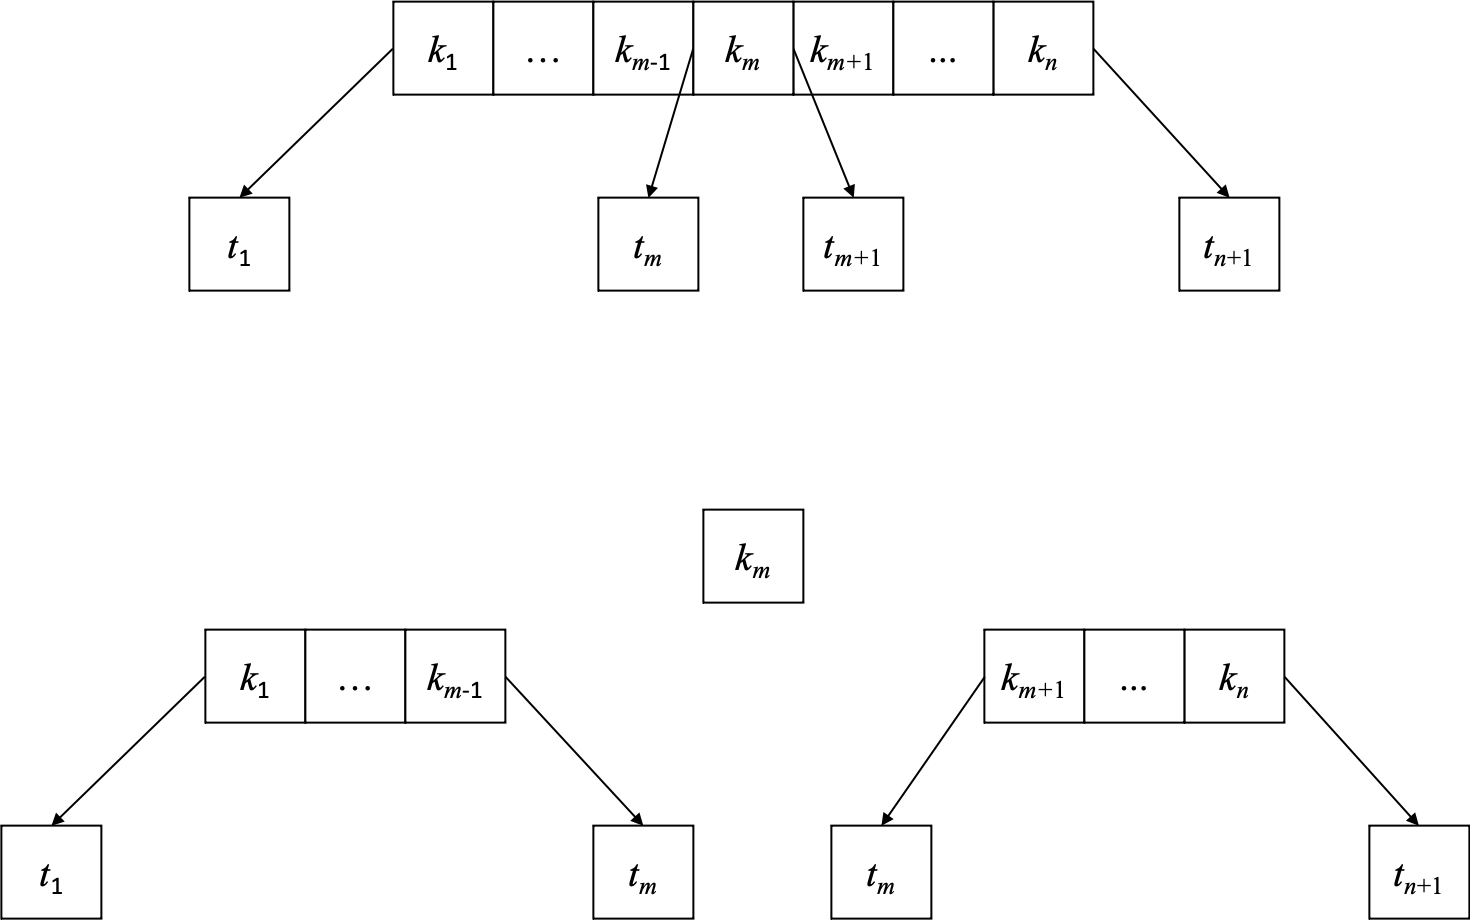
\includegraphics[scale=0.4]{img/split}
  \caption{Split the node into 3 parts at $m$}
  \label{fig:node-split}
\end{figure}

\be
split\ m\ (ks, ts) = ((ks_l, ts_l), k, (ks_r, ts_r))
\ee

We reuse the list $splitAt$ function defined in \cref{eq:split-at} in chapter 1 to realize it.

\[
\begin{cases}
(ks_l, (k:ks_r)) & = splitAt\ (m - 1)\ ks \\
(ts_l, ts_r) & = splitAt\ m\ ts
\end{cases}
\]

We can define the reversed operation $unsplit$ to combine the 3 parts back into a B-tree node.

\be
unsplit\ (ks_l, ts_l)\ k\ (ks_r, ts_r) = (ks_l \doubleplus [k] \doubleplus ks_r, ts_l \doubleplus ts_r)
\label{eq:btree-unsplit}
\ee

Below function first inserts $x$ to the tree $t$, then calls $fix$ to resume the B-tree balance rules with the given degree $d$.

\be
insert\ x\ (d, t) = fix\ (d, ins\ t)
\ee

After $ins$, if the root contains too many keys, function $fix$ calls $split$ to break it and build a new root.

\be
fix\ (d, t) = \begin{cases}
  full\ d\ t : & (d, ([k], [l, r])), \text{where}\ (l, k, r) = split\ d\ t \\
  otherwise  : & (d, t)
\end{cases}
\ee

$ins$ need handle two cases: for leaf node, we can reuse the list ordered $insert$ function defined in \cref{eq:list-ordered-insert} in chapter 1; otherwise, we need find the position to recursively insert to sub-tree. To do that, we define a $partition$ function as:

\be
partition\ x\ (ks, ts) = (l, t', r)
\ee

Where $l = (ks_l, ts_l)$ and $r = (ks_r, ts_r)$. It further uses the list partition function $span$ defined in \cref{eq:span} in chapter 1:

\[
\begin{cases}
(ks_l, ks_r) & = span\ (< x)\ ks \\
(ts_l, (t':ts_r)) & = splitAt\ |ks_l|\ ts
\end{cases}
\]

As such, we separate all the keys and sub-trees less than $x$ on the left as $l$, and those greater than $x$ on the right as $r$. The last sub-tree that less than $x$ is extracted as $t'$. We then recursively insert $x$ to $t'$, as shown in \cref{fig:recursive-insert}.

\be
\begin{array}{rcll}
  ins\ (ks, \nil) & = & (insert_L\ x\ ks, \nil) & \text{list insert for leaf}\\
  ins\ (ks, ts)   & = & balance\ d\ l\ (ins\ t')\ r & \text{where}\ (l, t', r) = partition\ x\ t \\
\end{array}
\ee

\begin{figure}[htbp]
  \centering
  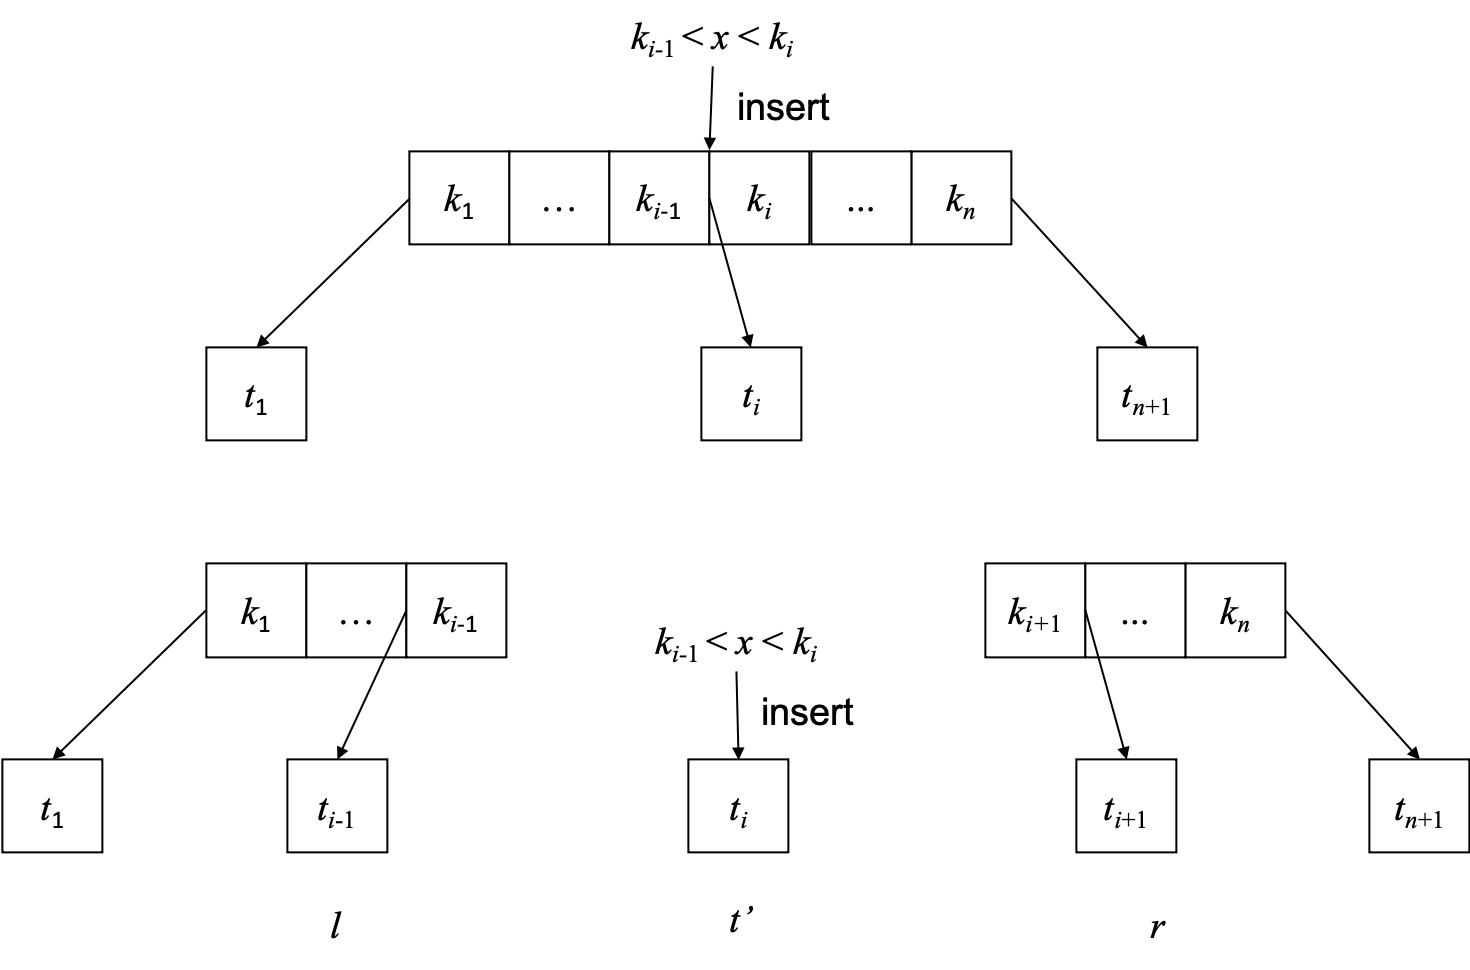
\includegraphics[scale=0.45]{img/partition}
  \caption{partition a node with $x$}
  \label{fig:recursive-insert}
\end{figure}

After insert $x$ to $t'$, it may contains too many keys that violates B-tree rules. We define function $balance$ to recursively recover B-tree rules by splitting sub-tree.

\be
balance\ d\ (ks_l, ts_l)\ t\ (ks_r, ts_r) = \begin{cases}
  full\ d\ t: fix_f \\
  otherwise: (ks_l \doubleplus ks_r, ts_l \doubleplus [t] \doubleplus ts_r)
  \end{cases}
\ee

where $fix_f$ splits sub-tree $t$ with degree $d$ as $(t_1, k, t_2) = split\ d\ t$, then combine them to a new B-tree node:

\be
fix_f = (ks_l \doubleplus [k] \doubleplus ks_r, ts_l \doubleplus [t_1, t_2] \doubleplus ts_r)
\ee

The following example program implements $insert$ for B-tree.

\begin{Haskell}
partition x (BTree ks ts) = (l, t, r) where
  l = (ks1, ts1)
  r = (ks2, ts2)
  (ks1, ks2) = span (< x) ks
  (ts1, (t:ts2)) = splitAt (length ks1) ts

split d (BTree ks ts) = (BTree ks1 ts1, k, BTree ks2 ts2) where
  (ks1, k:ks2) = splitAt (d - 1) ks
  (ts1, ts2) = splitAt d ts

insert x (d, t) = fixRoot (d, ins t) where
    ins (BTree ks []) = BTree (List.insert x ks) []
    ins t = balance d l (ins t') r where (l, t', r) = partition x t

fixRoot (d, t) | full d t  = let (t1, k, t2) = split d t in
                               (d, BTree [k] [t1, t2])
               | otherwise = (d, t)

balance d (ks1, ts1) t (ks2, ts2)
    | full d t  = fixFull
    | otherwise = BTree (ks1 ++ ks2) (ts1 ++ [t] ++ ts2)
  where
    fixFull = let (t1, k, t2) = split d t in
                BTree (ks1 ++ [k] ++ ks2) (ts1 ++ [t1, t2] ++ ts2)
\end{Haskell}

\Cref{fig:btree-insert-fp} shows the example B-trees built by repeatedly insert elements from list ``GMPXACDEJKNORSTUVYZ''.

\begin{figure}[htbp]
  \centering
  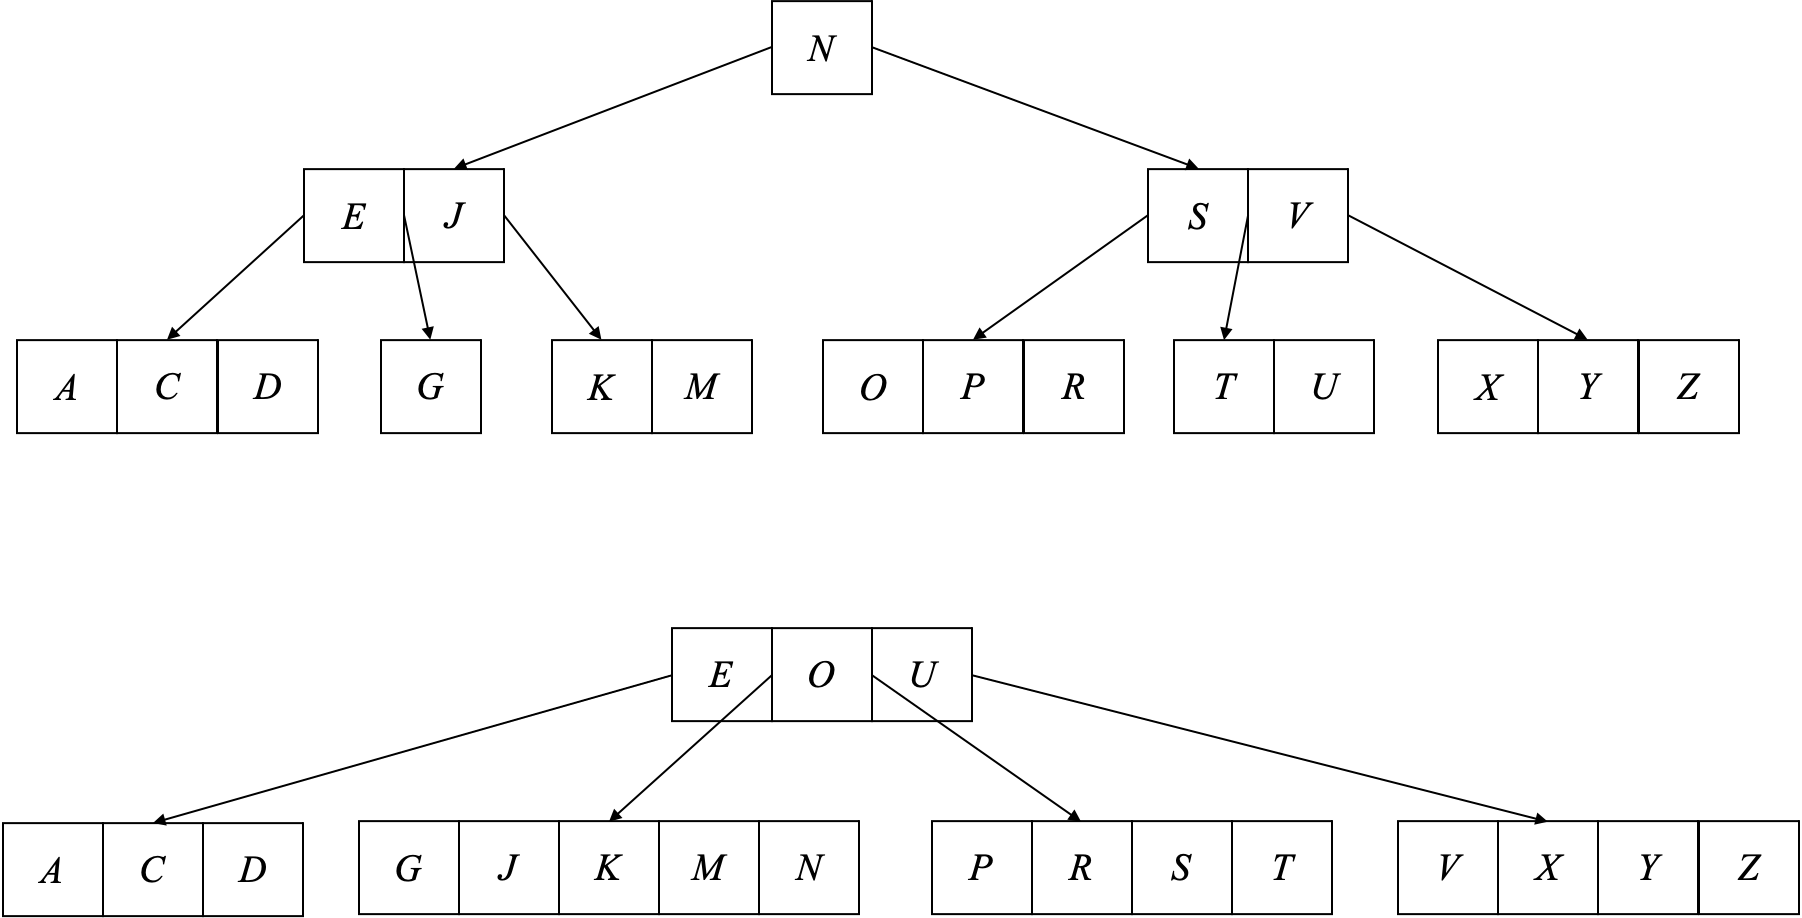
\includegraphics[scale=0.4]{img/btree-insert-fp}
  \caption{Repeatedly insert elements from ``GMPXACDEJKNORSTUVYZ''. above: $d = 2$ (2-3-4 tree), below: $d = 3$}
  \label{fig:btree-insert-fp}
\end{figure}

\subsection{Split before insert}

The second method is to split a node before insertion to prevent it becoming overly full. We often see this method in imperative implementations. When perform top-down recursive insert, if we reach to a node with $2d - 1$ keys, we divide it into 3 parts as shown in \cref{fig:node-split}, such that each new node has $d - 1$ keys. They will be valid B-tree node after insertion. For node $x$, let $K(x)$ be the keys, $T(x)$ be the sub-trees. Denote the $i$-th key of $x$ as $k_i(x)$, the $j$-th sub-tree as $t_j(x)$. Below algorithm splits the $i$-th sub-tree of node $z$:

\begin{algorithmic}[1]
\Procedure{Split}{$z, i$}
  \State $d \gets$ \Call{Deg}{$z$}
  \State $x \gets t_i(z)$
  \State $y \gets$ \Call{Create-Node}{}
  \State $K(y) \gets [k_{d + 1}(x), k_{d + 2}(x), ..., k_{2d - 1}(x)]$
  \State $K(x) \gets [k_1(x), k_2(x), ..., k_{d-1}(x)]$
  \If{$x$ is not leaf}
    \State $T(y) \gets [t_{d + 1}(x), t_{d + 2}(x), ..., t_{2d}(x)]$
    \State $T(x) \gets [t_1(x), t_2(x), ..., t_d(x)]$
  \EndIf
  \State \Call{Insert-At}{$K(z), i, k_d(x)$}
  \State \Call{Insert-At}{$T(z), i + 1, y$}
\EndProcedure
\end{algorithmic}

When split the node $x = t_i(z)$, we push the $d$-th key $k_d(x)$ up to the parent node $z$. If $z$ is already full, the pushing will break B-tree rules. To solve this problem, we need do the top-down check from the root along the path when insert. Split any node with $2d - 1$ keys. Since all parent nodes are processed to be not full, they can accept the additional key pushed up. This method needs one single pass down the tree without any back-tracking. If the root is full, we create a new node, and put the root as it singleton sub-tree. Below is the insert algorithm:

\begin{algorithmic}[1]
\Function{Insert}{$t, k$}
  \State $r \gets t$
  \If{$r$ is full} \Comment{root is full}
    \State $s \gets$ \Call{CREATE-NODE}{}
    \State $T(s) \gets [ r ]$
    \State \Call{Split}{$s, 1$}
    \State $r \gets s$
  \EndIf
  \State \Return \Call{Insert-Nonfull}{$r, k$}
\EndFunction
\end{algorithmic}

Where \textproc{Insert-Nonfull} assumes the node $r$ passed in
is not full. If $r$ is a leaf, we insert $k$ to the keys based on order (\Cref{ex:btree-binary-search} asks to realize the ordered insert with binary search); otherwise, we locate the position, where $k_i(r) < k < k_{i+1}(r)$. Split the sub-tree $t_i(r)$ if it is full, and go on insert to this sub-tree.

\begin{algorithmic}[1]
\Function{Insert-Nonfull}{$r, k$}
  \State $n \gets |K(r)|$
  \If{$r$ is leaf}
    \State $i \gets 1$
    \While{$i \leq n$ and $k > k_i(r)$}
      \State $i \gets i + 1$
    \EndWhile
    \State \Call{Insert-At}{$K(r), i, k$}
  \Else
    \State $i \gets n$
    \While{$i > 1$ and $k < k_i(r)$}
      \State $i \gets i - 1$
    \EndWhile
    \If{$t_i(r)$ is full}
      \State \Call{Split}{$r, i$}
      \If{$k > k_i(r)$}
        \State $i \gets i + 1$
      \EndIf
    \EndIf
    \State \Call{Insert-Nonfull}{$t_i(r), k$}
  \EndIf
  \State \Return $r$
\EndFunction
\end{algorithmic}

This algorithm is recursive. \Cref{ex:btree-loop-insert} asks to eliminate the recursion with pure loops. \Cref{fig:btree-insert} gives the result with the same input of ``GMPXACDEJKNORSTUVYZ''.

\begin{figure}[htbp]
  \centering
  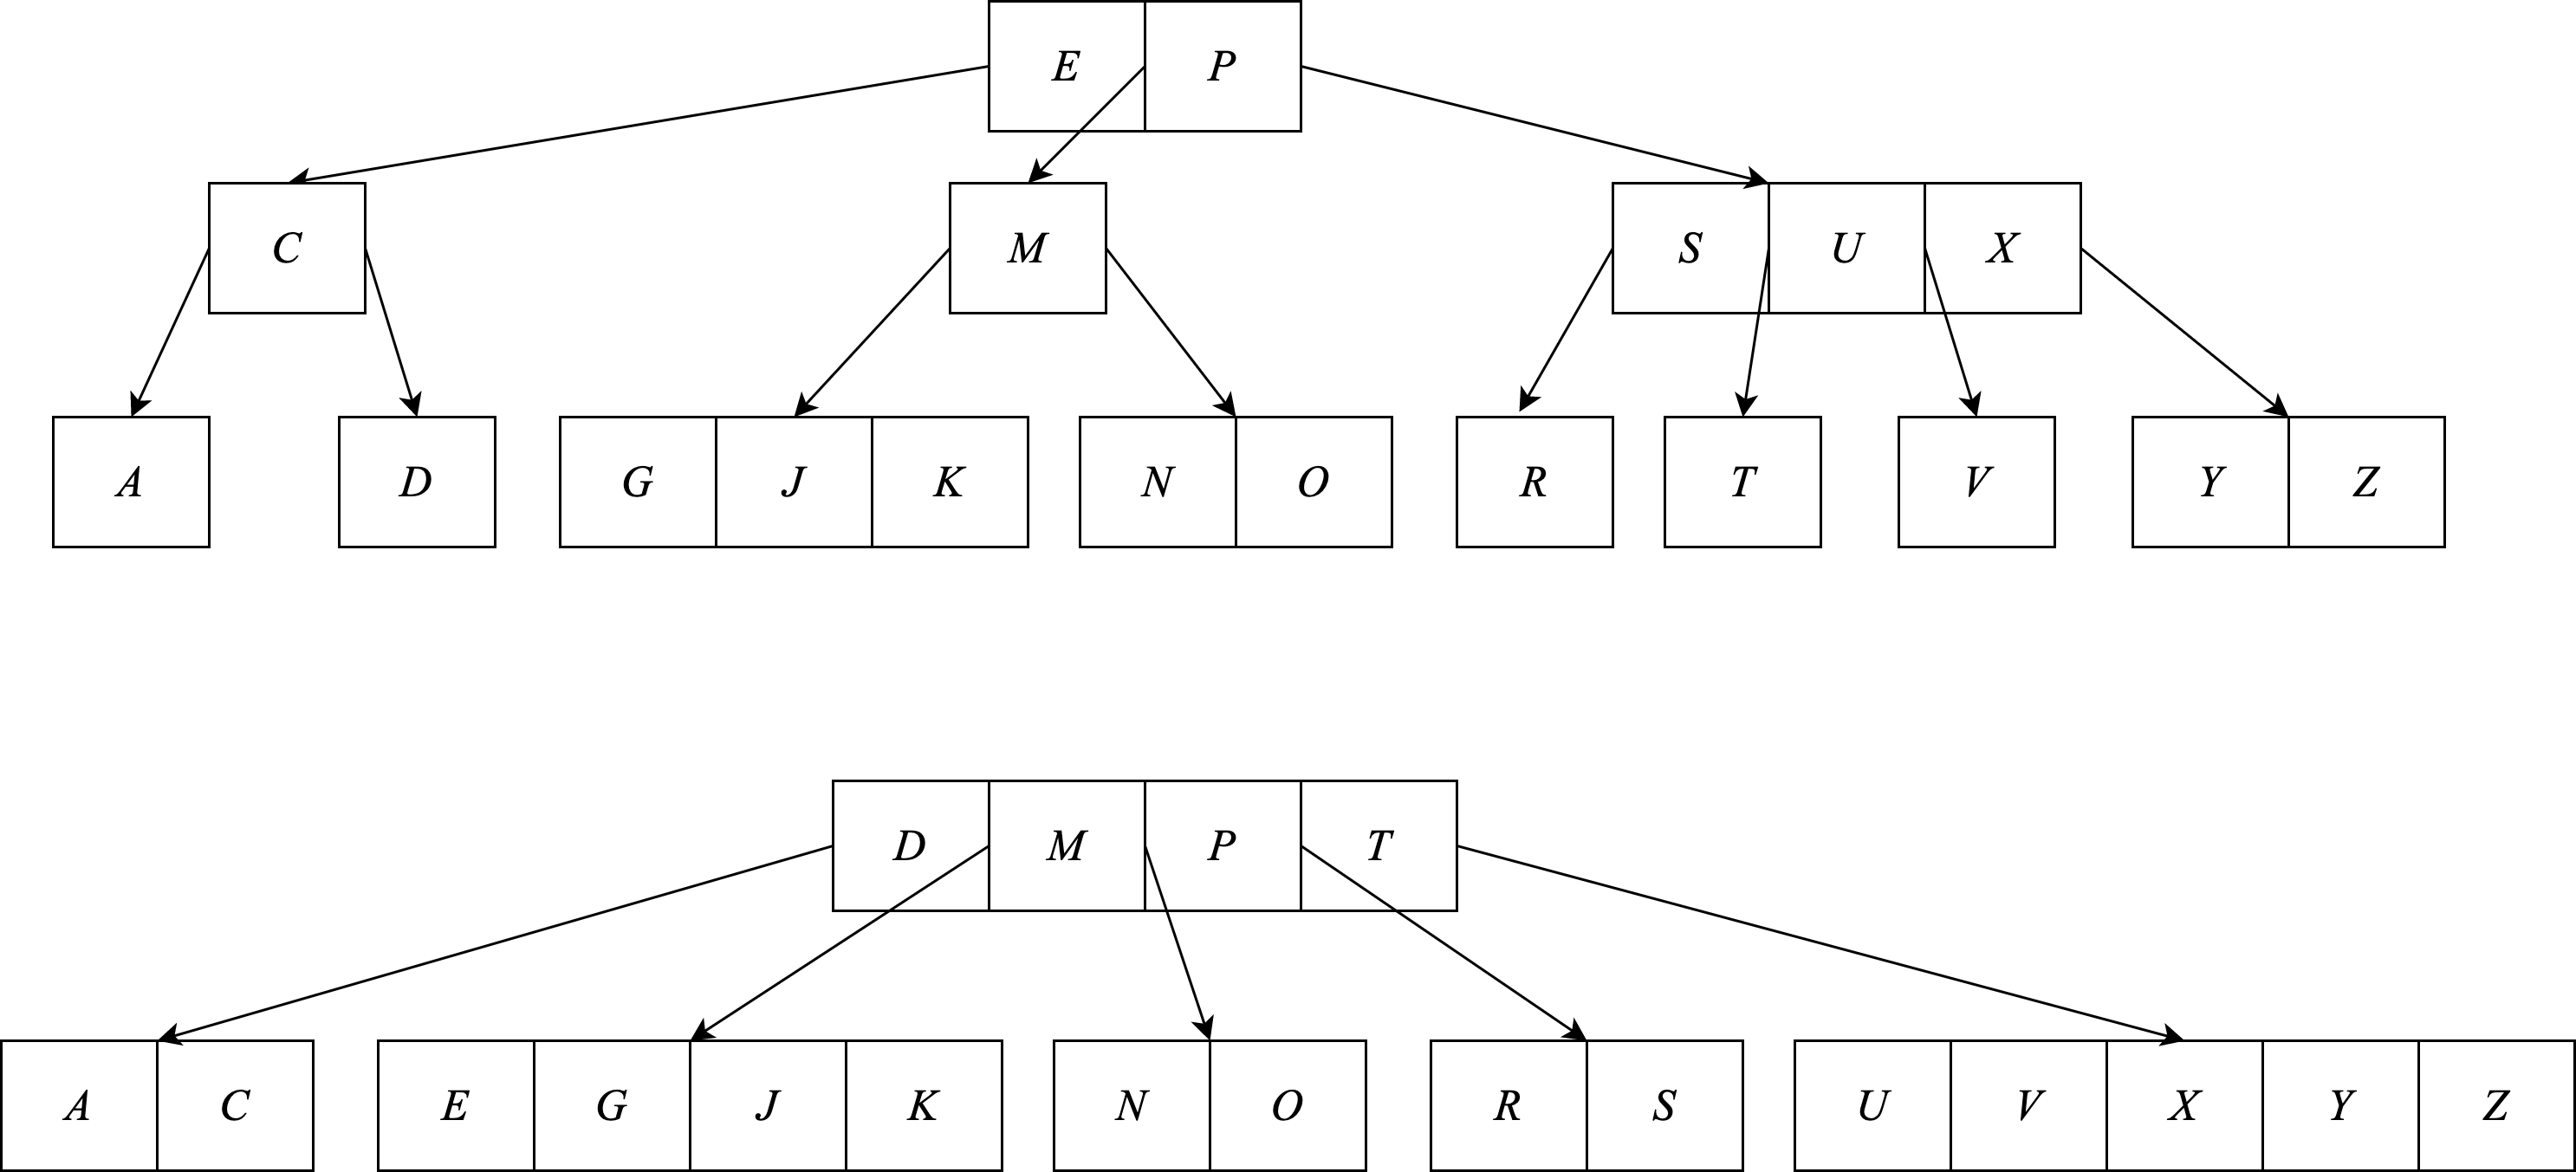
\includegraphics[scale=0.5]{img/btree-split-insert-example}
  \caption{Insert from ``GMPXACDEJKNORSTUVYZ''. up: $d = 2$, 2-3-4 tree; bottom: $d = 3$.}
  \label{fig:btree-insert}
\end{figure}

\subsection{Paired lists}

When use list to store ordered keys, we always start from the first key, and scan the list to find the insert position. If the keys are stored in array, we can improve it with binary search. Can we start somewhere in the node, go left or right depending on the order of keys? One idea is to separate the B-tree node into three parts: left $l$, a sub-tree $t'$, and right $r$. Where left and right are lists of pairs, each pair contains a key and a sub-tree: $(k_i, t_i)$. However, $l$ is reversed. In other words, $l$ and $r$ are head-to-head connected by $t'$ as a U-shape shown in \cref{fig:paired-lists}. We can move forward and backward both in constant time.

\begin{figure}[htbp]
  \centering
  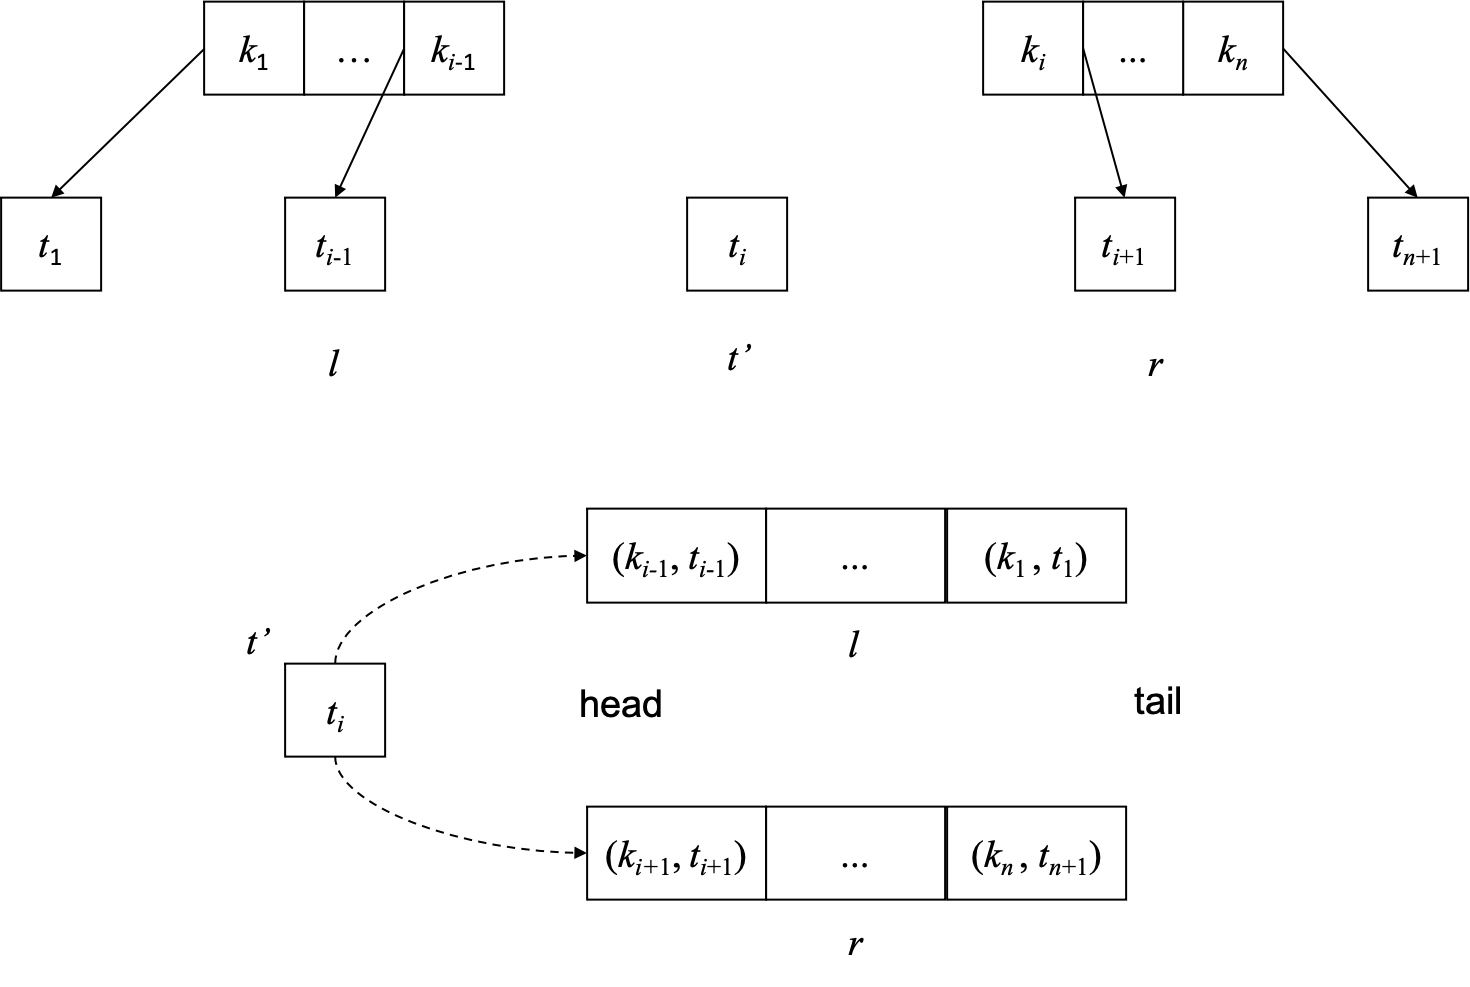
\includegraphics[scale=0.45]{img/paired-lists}
  \caption{Define the B-tree node with a sub-tree and paired lists}
  \label{fig:paired-lists}
\end{figure}

Below example program defines B-tree node. It's either empty, or contains 3 parts: the left (key, sub-tree) list in reversed order, a sub-tree, and the right (key, sub-tree) list. We denoted the none empty node as $(l, t', r)$.

\begin{Haskell}
data BTree a = Empty
           | BTree [(a, BTree a)] (BTree a) [(a, BTree a)]
\end{Haskell}

When move to right by a step, we take the first pair $(k, t)$ from $r$, then form another pair $(k, t')$ in front of $l$, and replace $t'$ with $t$. When move to left a step, it is symmetric. Both operations take constant time.

\be
\begin{array}{lcl}
  step_l\ ((k, t):l, t', r) & = & (l, t, (k, t'):r) \\
  step_r\ (l, t', (k, t):r) & = & ((k, t'):l, t, r) \\
\end{array}
\ee

With the left/right moves, we can implement a generic partition function $partition\ p\ t$, that separates the tree $t$ with a given predicate $p$ into 3 parts: left, middle, right: $(l, m, r)$, such that all sub-trees in $l$ and $m$ satisfy $p$, while the sub-trees in $r$ do not. Let the function $hd = fst \circ head$, which picks the first pair $(a, b)$ from a list, then extracts $a$ out.

\be
\begin{array}{lcl}
  partition\ p\ (\nil, m, r) & = & \begin{cases}
    p(hd(r)): & partition\ p\ (step_r\ t) \\
    otherwise: & (\nil, m, r) \\
  \end{cases} \\
  partition\ p\ (l, m, \nil) & = & \begin{cases}
    (not \circ p)(hd(l)): & partition\ p\ (step_l\ t) \\
    otherwise: & (l, m, \nil) \\
  \end{cases}\\
  partition\ p\ (l, m, r) & = & \begin{cases}
    p(hd(l))\ \text{and}\ (not \circ p)(hd(r)): & (l, m, r) \\
    p(hd(r)): & partition\ p\ (step_r\ t) \\
    (not \circ p)(hd(l)): & partition\ p\ (step_l\ t) \\
  \end{cases}
\end{array}
\ee

For example, $partition\ (<k)\ t$ moves all keys and sub-trees in $t$ less than $k$ out of the right part. Below example program implements the $partition$ function:

\begin{Haskell}
partition p t@(BTree [] m r)
  | p (hd r) = partition p (stepR t)
  | otherwise = ([], m, r)
partition p t@(BTree l m [])
  | (not . p) (hd l) = partition p (stepL t)
  | otherwise = (l, m, [])
partition p t@(BTree l m r)
  | p (hd l) && (not . p) (hd r) = (l, m, r)
  | p (hd r) = partition p (stepR t)
  | (not . p) (hd l) = partition p (stepL t)
\end{Haskell}

We can also use $step_l/step_r$ to split a B-tree at position $d$ when it becomes overly full. Let $n = |l|$ be the number of keys/sub-trees of the left part. $f^n(x)$ means repeatedly apply function $f$ to $x$ for $n$ times.

\be
split\ d\ t = \begin{cases}
  n < d: & sp(step_r^{d - n}(t)) \\
  n > d: & sp(step_r^{n - d}(t)) \\
  otherwise: & sp(t) \\
  \end{cases}
\ee

Where $sp$ does the separation work as below:

\be
sp\ (l, t, (k, t'):r) = ((l, t, \nil), k, (\nil, t', r))
\ee

With $partition$ and $split$ defined, we can define B-tree insert algorithm for the paired lists implementation. Firstly, we need modify the low/full testing to count both left and right parts:

\be
\begin{array}{ll}
  full\ d\ \nil & = False \\
  full\ d\ (l, t', r) & = |l| + |r| > 2d - 1 \\
\end{array}
\ee
and
\be
\begin{array}{ll}
  low\  d\ \nil & = False \\
  low\  d\ (l, t', r) & = |l| + |r| < d - 1 \\
\end{array}
\ee

When insert key $x$ to B-tree $t$ of degree $d$, we do the recursive insertion, then fix the root if it gets overly full:

\be
insert\ x\ (d, t) = fix\ (d, ins\ t)
\ee

Where $fix$ splits the root at $d$ if needed:

\be
fix\ (d, t) = \begin{cases}
  full\ d\ t: & (d, (\nil, t_1, [(k, t_2)]\ \text{where}\ (t_1, k, t_2) = split\ d\ t \\
  otherwise: & (d, t)
  \end{cases}
\ee

Function $ins$ need handle both $t = \nil$, and $t \neq \nil$ cases. For empty case, we create a singleton leaf; otherwise, we call $(l, t', r) = partition\ (< x)\ t$ to locate the position for recursive insert:

\be
\begin{array}{lcl}
  ins\ \nil & = & (\nil, \nil, [(x, \nil)]) \\
  ins\ t & = & \begin{cases}
    t' = \nil: & balance\ d\ l\ \nil\ ((x, \nil):r) \\
    t' \neq \nil: & balance\ d\ l\ (ins\ t')\ r \\
  \end{cases}
\end{array}
\ee

Function $balance$ examines if the sub-tree $t$ contains too many keys, and splits it.

\be
balance\ d\ l\ t\ r = \begin{cases}
  full\ d\ t: & fixFull \\
  otherwise: & (l, t, r)
  \end{cases}
\ee

Where $fixFull = (l, t_1, ((k, t_2):r)$, and $(t_1, k, t_2) = split\ d\ t$. Below example program implements the insert algorithm:

\begin{Haskell}
insert x (d, t) = fixRoot (d, ins t) where
  ins Empty = BTree [] Empty [(x, Empty)]
  ins t = let (l, t', r) = partition (< x) t in
    case t' of
      Empty -> balance d l Empty ((x, Empty):r)
      _     -> balance d l (ins t') r

fixRoot (d, t) | full d t = let (t1, k, t2) = split d t in
                   (d, BTree [] t1 [(k, t2)])
               | otherwise = (d, t)

balance d l t r | full d t = fixFull
                | otherwise = BTree l t r
  where
    fixFull = let (t1, k, t2) = split d t in BTree l t1 ((k, t2):r)

split d t@(BTree l _ _) | n < d = sp $ iterate stepR t !! (d - n)
                        | n > d = sp $ iterate stepL t !! (n - d)
                        | otherwise = sp t
  where
    n = length l
    sp (BTree l t ((k, t'):r)) = (BTree l t [], k, BTree [] t' r)
\end{Haskell}

\begin{Exercise}
\Question{Can we use $\leq$ to support duplicated keys in B-Tree?} \label{ex:btree-leq}
\Question{For the `split then insert' algorithm, eliminate the recursion with loops.}
\label{ex:btree-loop-insert}
\Question{We use linear search among keys to find the proper insert position. Improve the imperative implementation with binary search. Is the big-O performance improved?}
\label{ex:btree-binary-search}
% No, is still linear, although the search speed up to O(\lg n), the insertion takes O(n) time to shift elements.
\end{Exercise}

\section{Look up}
\index{B-tree!look up}

For look up, we can extend from the binary search tree to multiple branches, and obtain the generic B-tree look up solution. There are only two directions when look up the binary search tree: left and right, while, there are multiple ways in B-tree. Consider look up $k$ in B-tree $t = (ks, ts)$, if $t$ is a leaf ($ts$ is empty), then the problem becomes list look up; otherwise, we partition the $t$ with $k$ into three parts: $l = (ks_l, ts_l), t', r = (ks_r, ts_r)$, where all keys in $l$ and sub-tree $t'$ are less then $k$, and the remaining ($\geq k$) is in $r$. If the first key in $ks_r$ equals $k$, then we find the answer; otherwise, we recursive look up in sub-tree $t'$.

\be
\begin{array}{lcl}
  lookup\ k\ (ks, \nil) & = & \begin{cases}
    k \in ks: & \textit{Just}\ (ks, \nil) \\
    otherwise: & \textit{Nothing}
  \end{cases} \\
  lookup\ k\ (ks, ts) & = & \begin{cases}
    \textit{Just}\ k = \textit{safeHd}\ ks_r: & \textit{Just}\ (ks, ts) \\
    otherwise: & lookup\ k\ t' \\
  \end{cases}\\
\end{array}
\ee

Where $((ks_l, ts_l), t', (ks_r, ts_r)) = partition\ k\ t$, and

\[
\begin{array}{lcl}
  \textit{safeHd}\ [] & = & \textit{Nothing} \\
  \textit{safeHd}\ (x:xs) & = & \textit{Just}\ x \\
\end{array}
\]

Below example program\footnote{\texttt{safeHd} is provided as \texttt{listToMaybe} in some library.} implements $lookup$.

\begin{Haskell}
lookup k t@(BTree ks []) = if k `elem` ks then Just t else Nothing
lookup k t = if (Just k) == safeHd ks then Just t
             else lookup k t'  where
  (_, t', (ks, _)) = partition k t
\end{Haskell}

For the paired list implementation, the idea is similar. If the tree is not empty, we partition it with the predicate `$< k$'. Then check if the first key in the right part equals to $k$, or recursively look up the partitioned sub-tree:

\be
\begin{array}{lcl}
  lookup\ k\ \nil & = & \textit{Nothing} \\
  lookup\ k\ t & = & \begin{cases}
    \textit{Just}\ k = \textit{safeFst}\ (\textit{safeHd}\ r): & \textit{Just}\ (l, t', r) \\
    otherwise: & lookup\ k\ t' \\
    \end{cases}
\end{array}
\ee

Where $(l, t', r) = partition\ (< k)\ t$ for the none empty tree case. \textit{safeFst} applies \textit{fst} function to a `Maybe' value. Below example program utilizes \textit{fmap} to do this:

\begin{Haskell}
lookup x Empty = Nothing
lookup x t = let (l, t', r) = partition (< x) t in
  if (Just x) == fmap fst (safeHd r) then Just (BTree l t' r)
  else lookup x t'
\end{Haskell}

For the imperative implementation, we start from the root $r$, find a position $i$ among the keys, such that $k_i(r) \leq k < k_{i+1}(r)$. If $k_i(r) = k$ then return the node $r$ and $i$ as a pair; otherwise, move to sub-tree $t_i(r)$ to go on looking up. If $r$ is a leaf and $k$ is not in the keys, then return nothing. It means $k$ does not exist in the tree.

\begin{algorithmic}[1]
\Function{Look-Up}{$r, k$}
  \Loop
    \State $i \gets 1, n \gets |K(r)|$
    \While{$i \leq n$ and $k > k_i(r)$}
      \State $i \gets i + 1$
    \EndWhile
    \If{$i \leq n$ and $k = k_i(r)$}
      \State \Return $(r, i)$
    \EndIf
    \If{$r$ is leaf}
      \State \Return Nothing \Comment{$k$ does not exist}
    \Else
      \State $r \gets t_i(r)$ \Comment{go to the $i$-th sub-tree}
    \EndIf
  \EndLoop
\EndFunction
\end{algorithmic}

\begin{Exercise}
  \Question{Improve the imperative look up with binary search among keys.}
\end{Exercise}

\section{Delete}
\index{B-tree!delete}

After delete a key, the number of keys may be too few to be a valid B-tree node. Except the root, the number of keys should not be less than $d - 1$, where $d$ is the minimum degree. There are two methods symmetric to insert: we can either delete then fix, or merge before delete.

\subsection{Delete and fix}

We first extend the $delete$ algorithm for binary search tree to multiple branches, then fix the B-tree balance rules. The main delete program is defined with these two steps:

\be
delete\ x\ (d, t) = fix (d, del\ x\ t)
\ee

Where function $del$ is the one we extend to support multiple branches. If $t$ is a leaf, we merely delete $x$ from the keys; otherwise, we partition the tree with $x$ into 3 parts: $(l, t', r)$. Where all the keys in $l$ and sub-tree $t'$ are less than $x$, and the rest in $r$ are great than or equal ($\geq$) to $x$. When $r$ isn't empty, we pick the first key $k_i$ from it. If the key equals to $x$, ($k_i = x$), we next replace it with the maximum key $k'$ of sub-tree $t'$ ($k' = max(t')$), and recursively delete $k'$ from $t'$ as shown in \cref{fig:btree-del}. Otherwise (either $r$ is empty, or $k_i \neq x$), we recursively delete $x$ from sub-tree $t'$.

\begin{figure}[htbp]
  \centering
  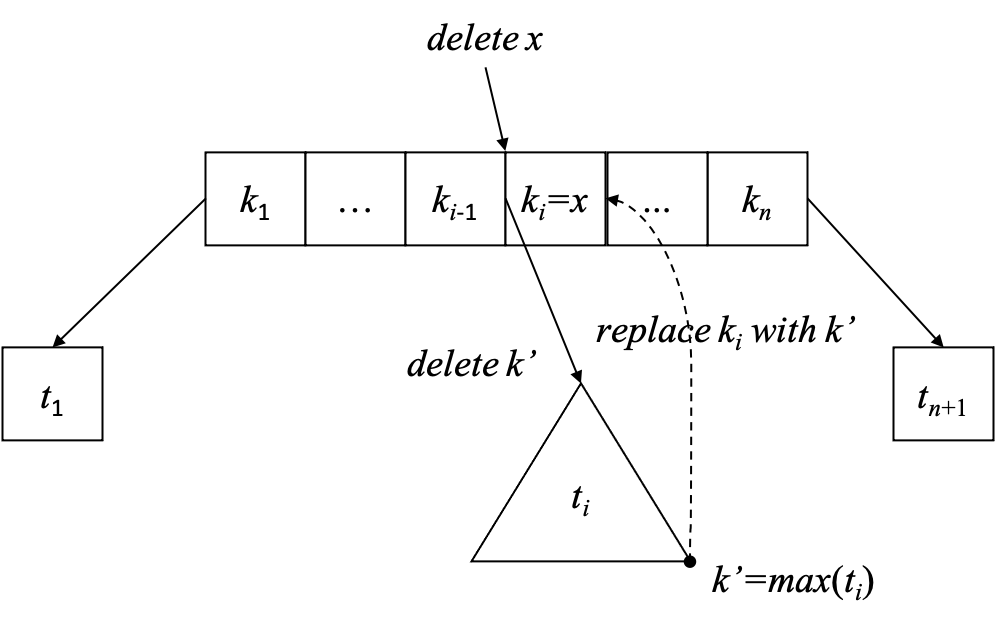
\includegraphics[scale=0.45]{img/btree-del}
  \caption{Replace $k_i$ with $k' = max(t')$, then recursively delete $k'$ from $t'$.}
  \label{fig:btree-del}
\end{figure}

\be
\begin{array}{lcl}
del\ x\ (ks, \nil) & = & (delete_l\ x\ ks, \nil) \\
del\ x\ t & = & \begin{cases}
  \textit{Just}\ x = \textit{safeHd}\ ks': & balance\ d\ l\ (del\ k'\ t')\ (k':(tail\ ks'), ts') \\
  otherwise: & balance\ d\ l\ (del\ x\ t')\ (ks', ts') \\
  \end{cases}
\end{array}
\ee

Where $(l, t', (ks', ts')) = partition\ x\ t$, are the 3 parts partitioned by $x$. On top of it, we extract the maximum key $k'$ from $t'$. The $max$ function is defined as:

\be
\begin{array}{lcl}
  max\ (ks, \nil) & = & last\ ks \\
  max\ (ks, ts) & = & max\ (last\ ts) \\
\end{array}
\ee

Function $last$ returns the last element from a list (\cref{eq:list-last} in chapter 1). $delete_l$ is the list delete algorithm (\cref{eq:list-delete} in chapter 1). $tail$ drops the first element from a list and returns the rest (\cref{eq:list-head-tail}). We need modify the $balance$ function, which we defined for $insert$ before, with the additional logic to merge the node if it contains too less keys.

\be
balance\ d\ (ks_l, ts_l)\ t\ (ks_r, ts_r) = \begin{cases}
  full\ d\ t: fix_f \\
  low\ d\ t: fix_l \\
  otherwise: (ks_l \doubleplus ks_r, ts_l \doubleplus [t] \doubleplus ts_r)
  \end{cases}
\ee

If $t$ is overly low ($< d - 1$ keys), we call $fix_l$ to merge it with the left part $(ks_l, ts_l)$ or right part $(ks_r, ts_r)$ depends on which side of keys is not empty. Use the left part for example: we extract the last element from $ks_l$ and $ts_l$ respectively, say $k_m$ and $t_m$. Then call $unsplit$ (defined in \cref{eq:btree-unsplit}) to merge them with $t$ as $unsplit\ t_m\ k_m\ t$. It forms a new sub-tree with more keys. Finally we call balance again to build the result B-tree.

\be
fix_l = \begin{cases}
  ks_l \neq \nil: & balance\ d\ (init\ ks_l, init\ ts_l)\ (unsplit\ t_m\ k_m\ t)\ (ks_r, ts_r) \\
  ks_r \neq \nil: & balance\ d\ (ks_l, ts_l)\ (unsplit\ t\ k_1\ t_1)\ (tail\ ks_r, tail\ ts_r) \\
  otherwise: & t
  \end{cases}
\ee

The last case (otherwise) means $ks_l = ks_r = \nil$, both sides are empty. The tree is a singleton leaf hence need not fixing. $k_1$ and $t_1$ are the first element in $ks_r$ and $ts_r$ respectively. Finally, we need modify the $fix$ function defined for $insert$, add new logic for $delete$:

\be
\begin{array}{lcl}
fix\ (d, (\nil, [t])) & = & (d, t) \\
fix\ (d, t) & = & \begin{cases}
  full\ d\ t : & (d, ([k], [l, r])), \text{where}\ (l, k, r) = split\ d\ t \\
  otherwise  : & (d, t)
\end{cases}
\end{array}
\ee

What we add is the first case. After delete, if the root contains nothing but a sub-tree, we can shrink the height, pull the single sub-tree as the new root. The following example program implements the $delete$ algorithm.

\begin{Haskell}
delete x (d, t) = fixRoot (d, del x t) where
    del x (BTree ks []) = BTree (List.delete x ks) []
    del x t = if (Just x) == safeHd ks' then
                let k' = max t' in
                   balance d l (del k' t') (k':(tail ks'), ts')
              else balance d l (del x t') r
      where
        (l, t', r@(ks', ts')) = partition x t

fixRoot (d, BTree [] [t]) = (d, t)
fixRoot (d, t) | full d t  = let (t1, k, t2) = split d t in
                               (d, BTree [k] [t1, t2])
               | otherwise = (d, t)

balance d (ks1, ts1) t (ks2, ts2)
    | full d t  = fixFull
    | low  d t  = fixLow
    | otherwise = BTree (ks1 ++ ks2) (ts1 ++ [t] ++ ts2)
  where
    fixFull = let (t1, k, t2) = split d t in
                BTree (ks1 ++ [k] ++ ks2) (ts1 ++ [t1, t2] ++ ts2)
    fixLow | not $ null ks1 = balance d (init ks1, init ts1)
                                      (unsplit (last ts1) (last ks1) t)
                                      (ks2, ts2)
           | not $ null ks2 = balance d (ks1, ts1)
                                      (unsplit t (head ks2) (head ts2))
                                      (tail ks2, tail ts2)
           | otherwise = t
\end{Haskell}

We leave the $delete$ function for the 'paired list' implementation as an exercise. \Cref{fig:btree-del-before, fig:btree-del-CJ, fig:btree-del-KN} give examples of delete.

\begin{figure}[htbp]
  \centering
  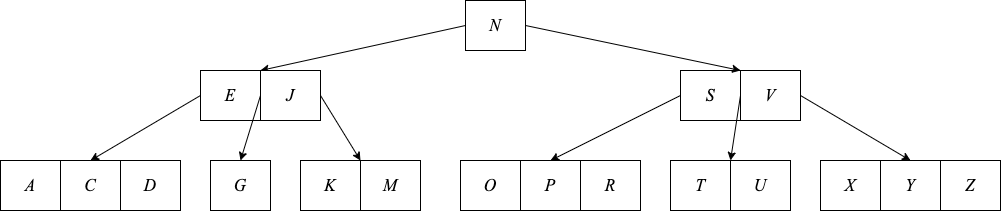
\includegraphics[scale=0.33]{img/btree-del-before}
  \caption{Before delete}
  \label{fig:btree-del-before}
\end{figure}

\begin{figure}[htbp]
  \centering
  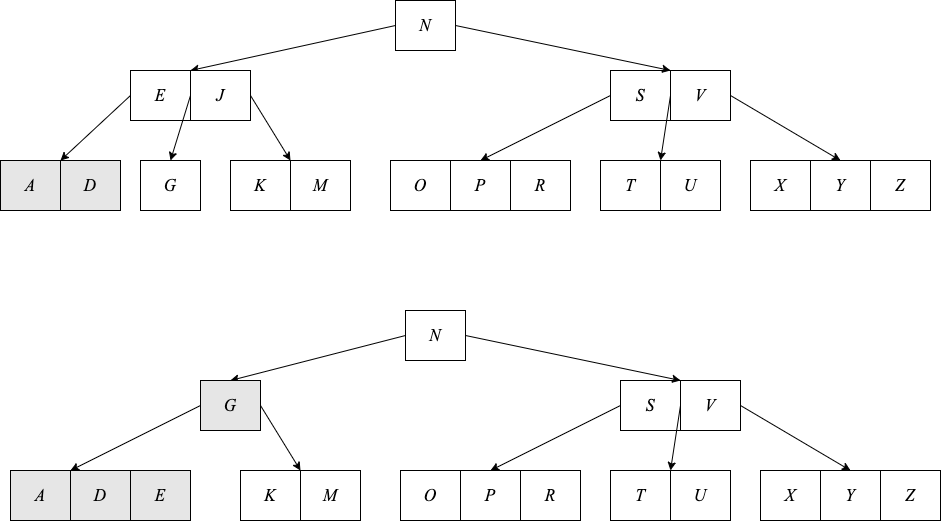
\includegraphics[scale=0.33]{img/btree-del-CJ}
  \caption{Delete `C', then delete `J'}
  \label{fig:btree-del-CJ}
\end{figure}

\begin{figure}[htbp]
  \centering
  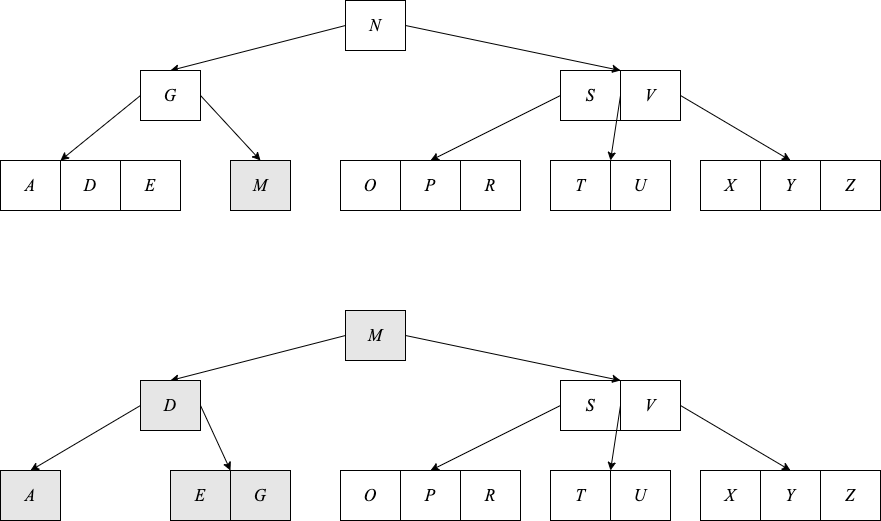
\includegraphics[scale=0.33]{img/btree-del-KN}
  \caption{Delete `K', then delete `N'}
  \label{fig:btree-del-KN}
\end{figure}

\subsection{Merge before delete}

The other way is to merge the nodes before delete if there are too few keys. Consider delete key $x$ from the tree $t$, let us start from the easy case.

\textbf{Case 1}. If $x$ exists in node $t$, and $t$ is a leaf, we can directly remove $x$ from $t$. If $t$ is the singleton node in the tree (root), we needn't worry about too few keys.

\textbf{Case 2}. If $x$ exists in node $t$, but $t$ is not a leaf. There are three sub-cases:

\textbf{Case 2a}. As shown in \cref{fig:btree-del}, let the predecessor of $k_i = x$ be $k'$, where $k' = max(t_i)$. If $t_i$ has sufficient keys ($\geq d$), we replace $k_i$ with $k'$, then recursively delete $k'$ from $t_i$.

\textbf{Case 2b}. If $t_i$ does not have enough keys, but the sub-tree $t_{i+1}$ does ($\geq d$). Symmetrically, we replace $k_i$ with its successor $k''$, where $k'' = min(t_{i+1})$, then recursively delete $k''$ from $t_{i+1}$, as shown in \cref{fig:btree-del-case2b}.

\begin{figure}[htbp]
  \centering
  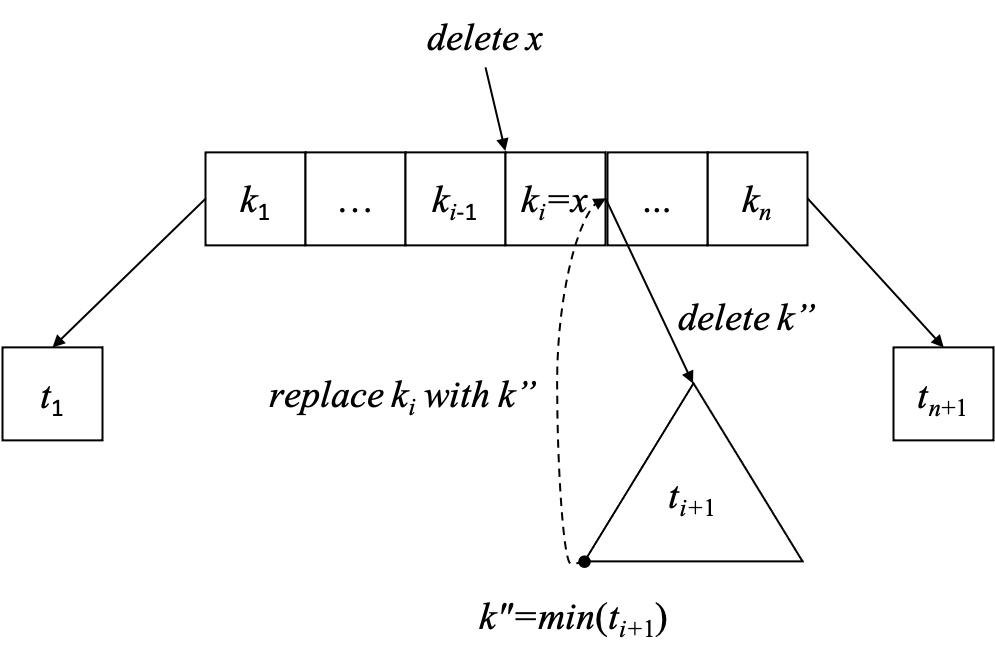
\includegraphics[scale=0.5]{img/btree-del-case2b}
  \caption{Replace $k_i$ with $k'' = min(t_{i+1})$, then delete $k''$ from $t_{i+1}$.}
  \label{fig:btree-del-case2b}
\end{figure}

\textbf{Case 2c}. If neither $t_i$ nor $t_{i+1}$ contains sufficient keys ($|t_i| = |t_{i+1}| = d - 1$), we merge $t_i, x, t_{i+1}$ to a new node. This new node has $2d - 1$ keys, we can safely perform delete on it as shown in \cref{fig:btree-del-merge}.

\begin{figure}[htbp]
  \centering
  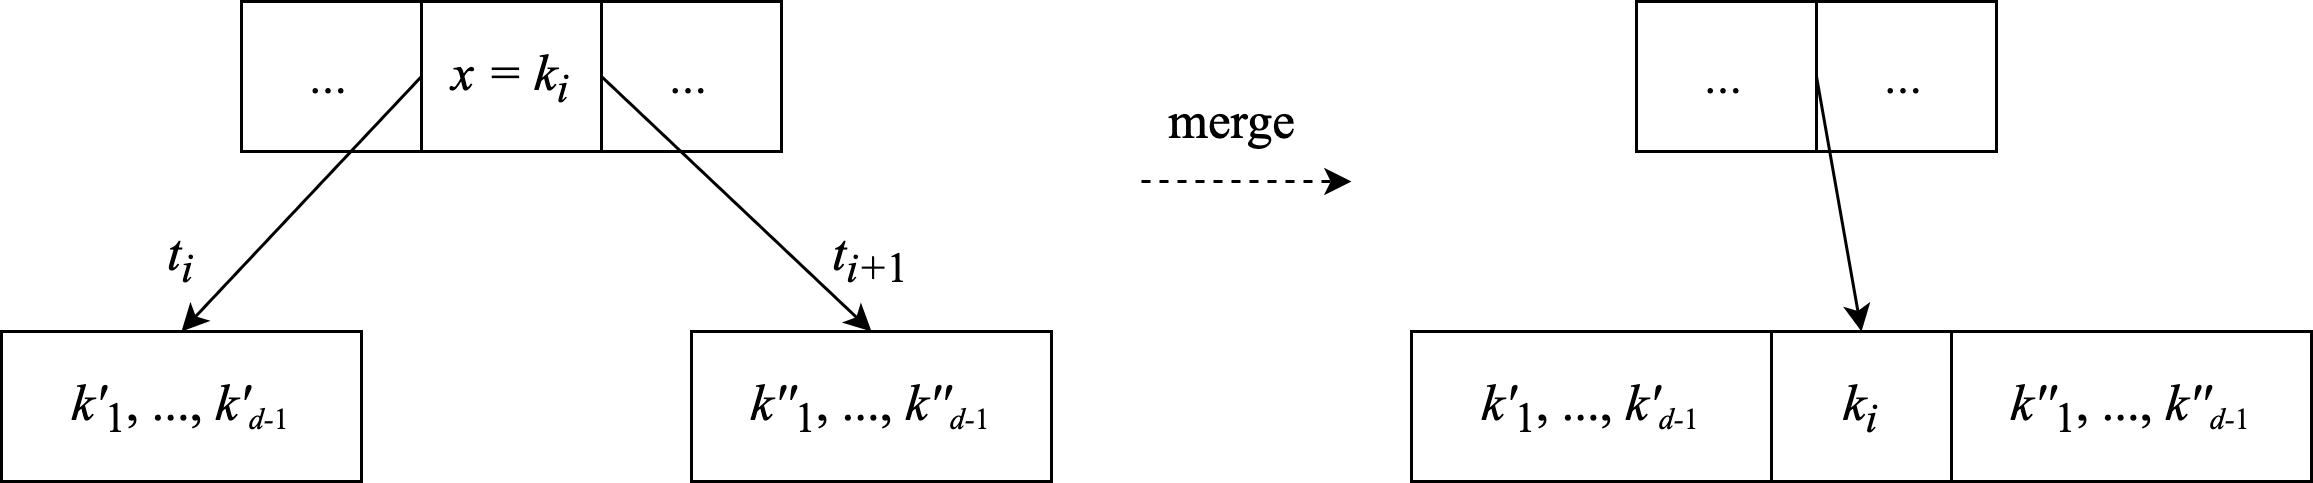
\includegraphics[scale=0.65]{img/btree-del-merge}
  \caption{Merge before delete}
  \label{fig:btree-del-merge}
\end{figure}

Merge pushes a key $k_i$ to the sub-tree. After that, if node $t$ becomes empty, it means $k_i$ is the only key in $t$, and $t_i, t_{i+1}$ are the only two sub-trees. We need shrink the tree height as shown in \cref{fig:btree-del-shrink}.

\begin{figure}[htbp]
  \centering
  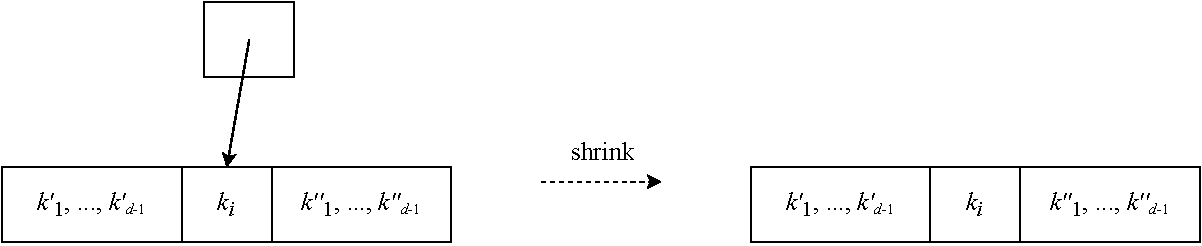
\includegraphics[scale=0.65]{img/btree-del-shrink}
  \caption{Shrink}
  \label{fig:btree-del-shrink}
\end{figure}

\textbf{Case 3}. If node $t$ does not contain $x$, we need recursively delete $x$ from a sub-tree $t_i$. There are two sub-cases if there are too few keys in $t_i$:

\textbf{Case 3a}. Among the two siblings $t_{i-1}, t_{i+1}$, if either one has enough keys ($\geq d$), we move a key from $t$ to $t_i$, then move a key from the sibling up to $t$, and move the corresponding sub-tree from the sibling to $t_i$. As shown in \cref{fig:btree-del-borrow}, $t_i$ received one more key. We next recursively delete $x$ from $t_i$.

\begin{figure}[htbp]
  \centering
  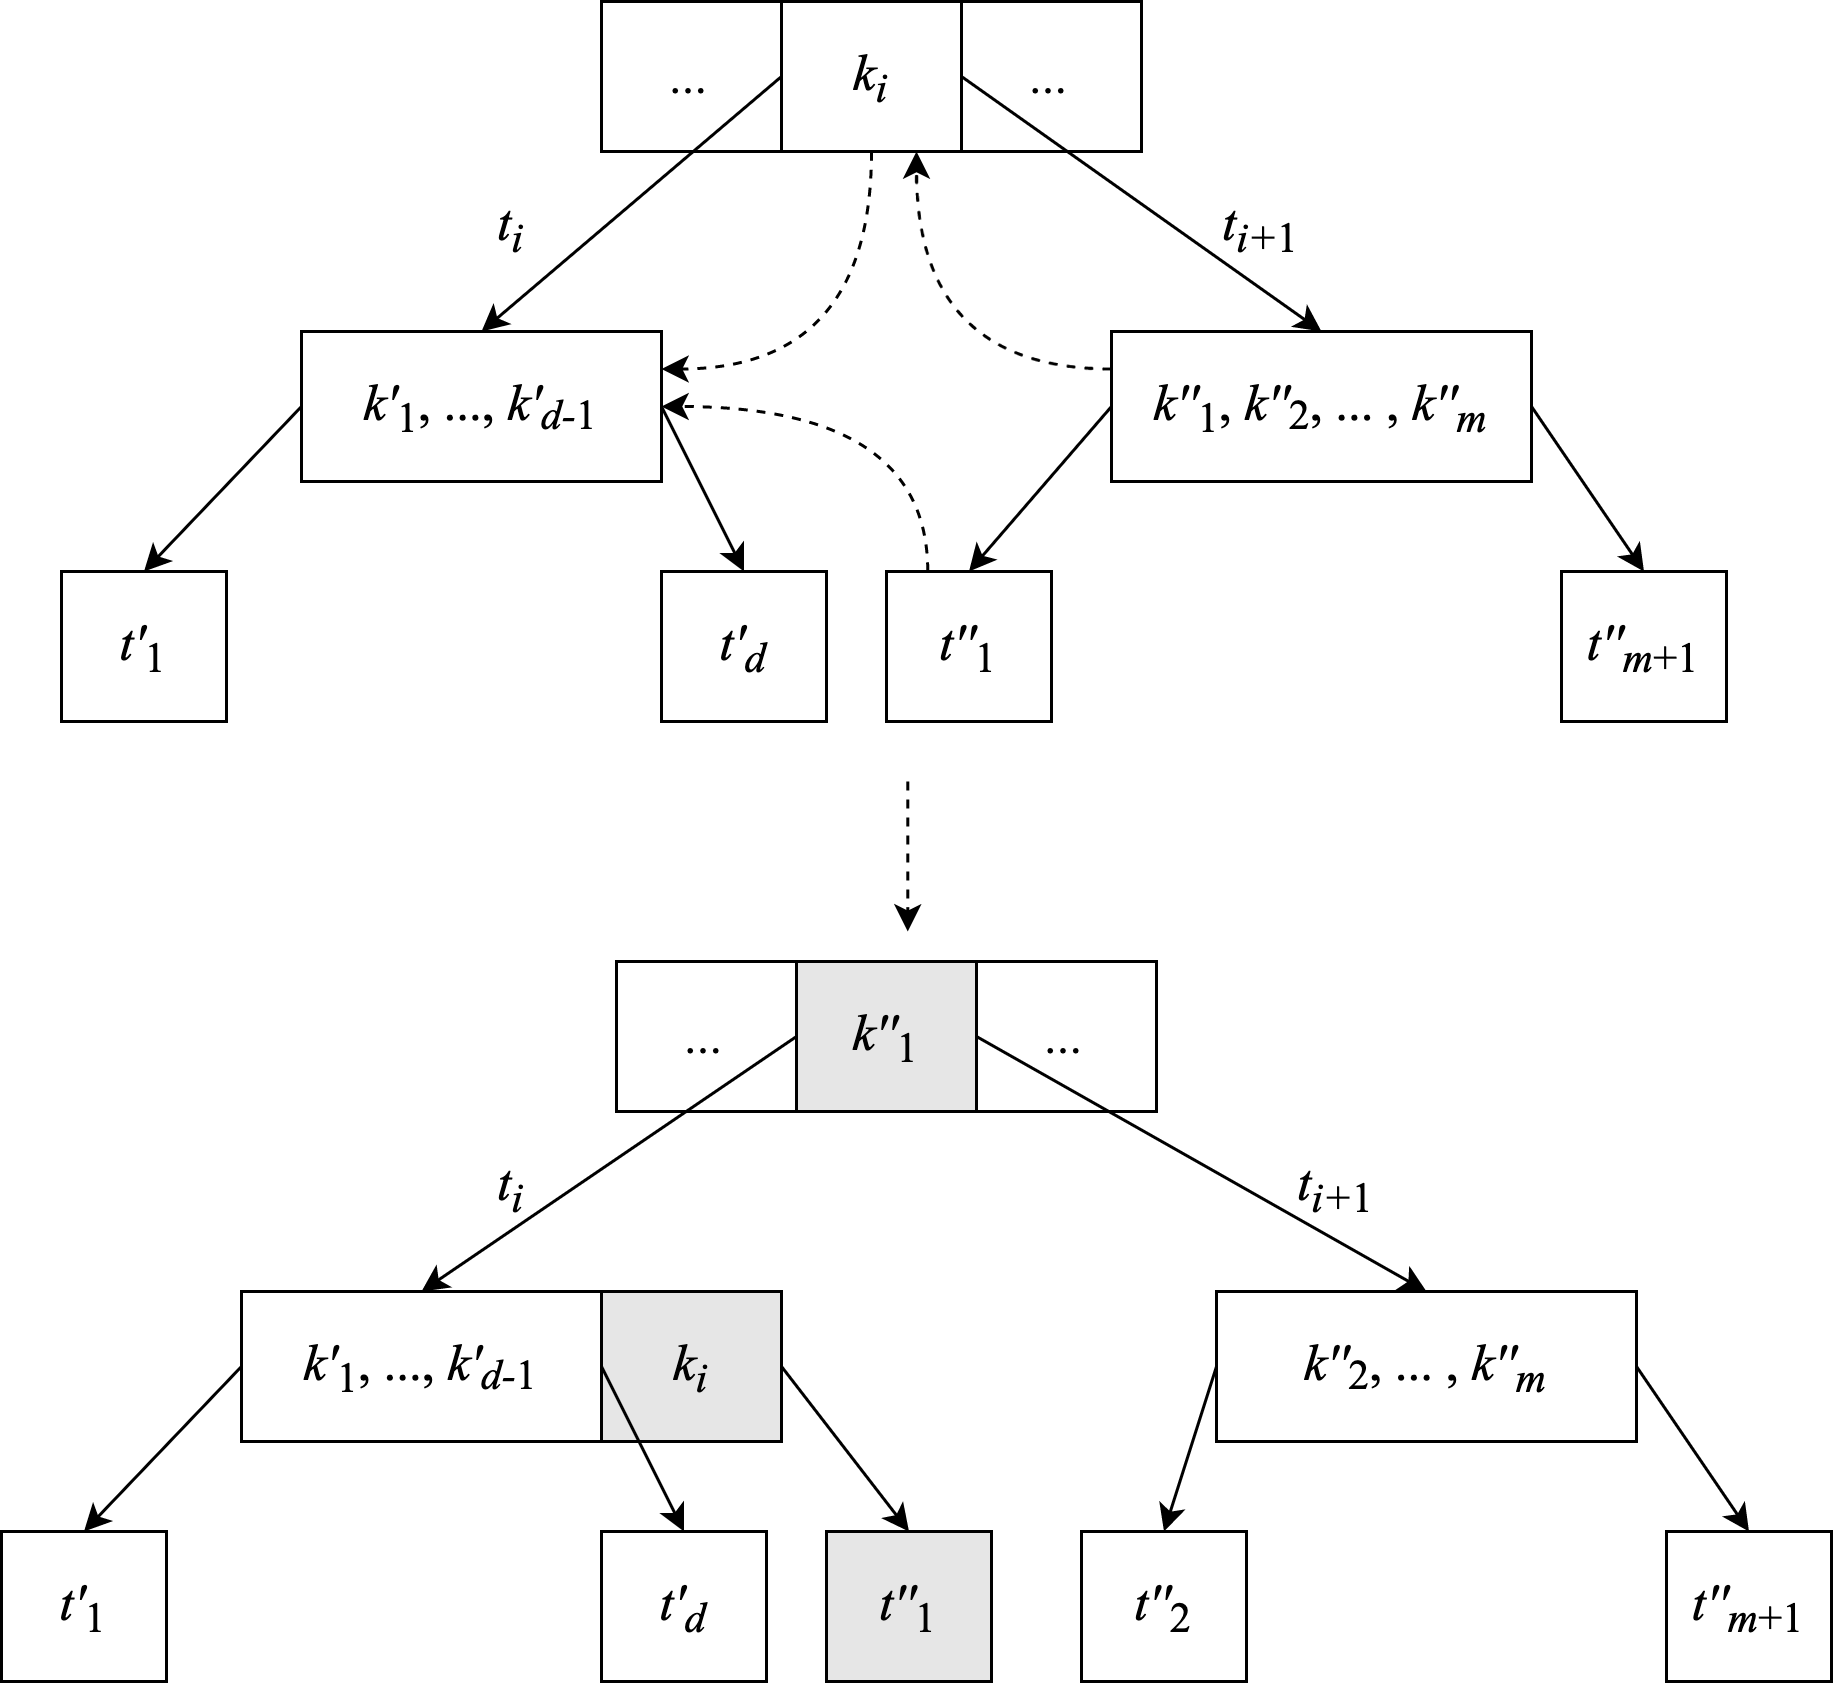
\includegraphics[scale=0.65]{img/btree-del-borrow}
  \caption{Borrow from the right sibling.}
  \label{fig:btree-del-borrow}
\end{figure}

\textbf{Case 3b}. If neither sibling has sufficient keys ($|t_{i-1}| = |t_{i+1}| = d - 1$), we merge $t_i$, a key from $t$, and either sibling into a new node, as shown in \cref{fig:btree-del-merge-subtree}. Then recursively delete $x$ from it.

\begin{figure}[htbp]
  \centering
  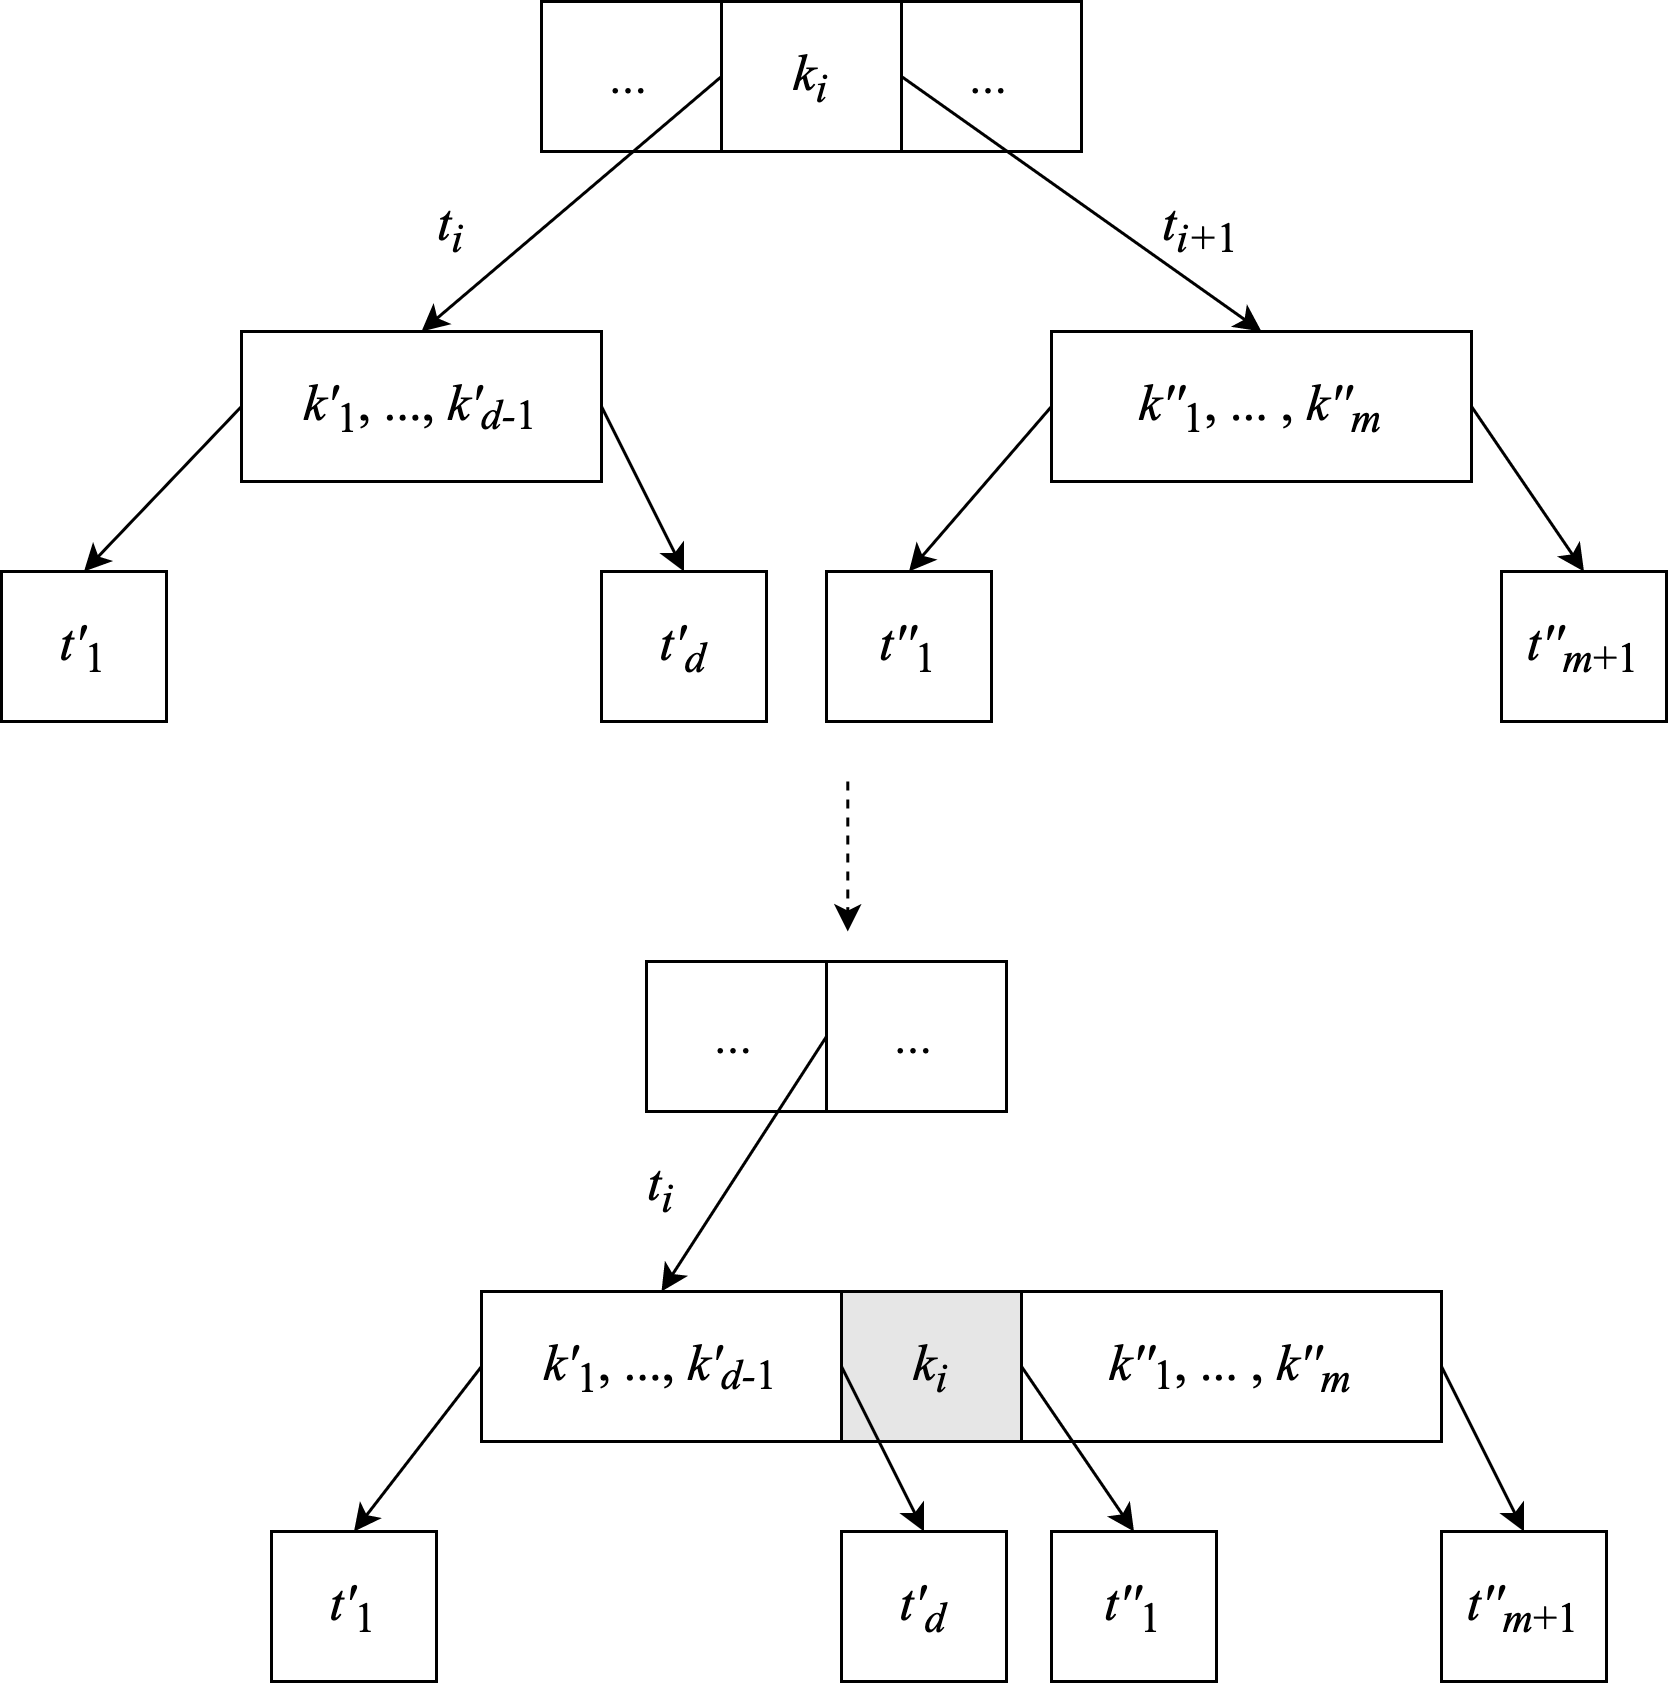
\includegraphics[scale=0.65]{img/btree-del-merge-subtree}
  \caption{Merge $t_i$, $k$, $t_{i+1}$}
  \label{fig:btree-del-merge-subtree}
\end{figure}

Below \textproc{Delete} algorithm implements the `merge then delete' method:

\begin{algorithmic}[1]
\Function{Delete}{$t, k$}
  \If{$t$ is empty}
    \State \Return $t$
  \EndIf
  \State $i \gets 1$, $n \gets |K(t)|$
  \While{$i \leq n$ and $k > k_i(t)$}
    \State $i \gets i + 1$
  \EndWhile
  \If{$k = k_i(t)$}
    \If{$t$ is leaf} \Comment{case 1}
      \State \Call{Remove}{$K(t), k$}
    \Else \Comment{case 2}
      \If{$|K(t_i(t))| \geq d$} \Comment{case 2a}
        \State $k_i(t) \gets$ \Call{Max}{$t_i(t)$}
        \State \Call{Delete}{$t_i(t), k_i(t)$}
      \ElsIf{$|K(t_{i+1}(t))| \geq d$} \Comment{case 2b}
        \State $k_i(t) \gets$ \Call{Min}{$t_{i+1}(t)$}
        \State \Call{Delete}{$t_{i+1}(t), k_i(t)$}
      \Else \Comment{case 2c}
        \State \Call{Merge-At}{$t, i$}
        \State \Call{Delete}{$t_i(t), k$}
        \If{$K(T)$ is empty}
          \State $t \gets t_i(t)$ \Comment{Shrinks height}
        \EndIf
      \EndIf
    \EndIf
    \State \Return $t$
  \EndIf
  \If{$t$ is not leaf}
    \If{$k > k_n(t)$}
      \State $i \gets i + 1$
    \EndIf
    \If{$|K(t_i(t))| < d$}  \Comment{case 3}
      \If{$i > 1$ and $|K(t_{i-1}(t))| \geq d$} \Comment{case 3a: left}
        \State \Call{Insert}{$K(t_i(t)), k_{i-1}(t)$}
        \State $k_{i-1}(t) \gets$ \Call{Pop-Last}{$K(t_{i-1}(t))$}
        \If{$t_i(t)$ is not leaf}
          \State \textproc{Insert}($T(t_i(t))$, \Call{Pop-Back}{$T(t_{i-1}(t))$})
        \EndIf
      \ElsIf{$i \leq n$ and $|K(t_{i+1}(t))| \geq d$} \Comment{case 3a: right}
        \State \Call{Append}{$K(t_i(t)), k_i(t)$}
        \State $k_i(t) \gets$ \Call{Pop-First}{$K(t_{i+1}(t))$}
        \If{$t_i(t)$ is not leaf}
          \State \textproc{Append}($T(t_i(t))$, \Call{Pop-First}{$T(t_{i+1}(t))$})
        \EndIf
      \Else \Comment{case 3b}
        \If{$i = n + 1$}
          \State $i \gets i - 1$
        \EndIf
        \State \Call{Merge-At}{$t, i$}
      \EndIf
    \EndIf
    \State \Call{Delete}{$t_i(t), k$}
    \If{$K(t)$ is empty} \Comment {Shrinks height}
      \State $t \gets t_1(t)$
    \EndIf
  \EndIf
  \State \Return $t$
\EndFunction
\end{algorithmic}

Where \textproc{Merge-At}($t, i$) merges sub-tree $t_i(t)$, key $k_i(t)$, and $t_{i+1}(t)$ into one sub-tree.

\begin{algorithmic}[1]
\Procedure{Merge-At}{$t, i$}
  \State $x \gets t_i(t)$
  \State $y \gets t_{i+1}(t)$
  \State $K(x) \gets K(x) \doubleplus [k_i(t)] \doubleplus K(y)$
  \State $T(x) \gets T(x) \doubleplus T(y)$
  \State \Call{Remove-At}{$K(t), i$}
  \State \Call{Remove-At}{$T(t), i+1$}
\EndProcedure
\end{algorithmic}

\begin{Exercise}
  \Question{When delete a key $k$ from the branch node, we use the maximum key from the predecessor sub-tree $k' = max(t')$ to replace $k$, then recursively delete $k'$ from $t'$. There is a symmetric method, to replace $k$ with the minimum key from the successor sub-tree. Implement this solution.}
  \Question{Define the $delete$ function for the `paired list' implementation.}
\end{Exercise}

\section{Summary}
We extend the binary search tree to multiple branches, then constrain the branches within a range to develop the B-tree. B-tree is used as a tool to control the magnetic disk access (chapter 18, \cite{CLRS}). Because all B-tree nodes store keys in a range, not too few or too many. B-tree is balanced. Most of the tree operations are proportion to the height. The performance is bound to $O(\lg n)$ time, where $n$ is the number of keys in B-tree.

\section{Appendix: Example programs}

Definition of B-tree:

\begin{lstlisting}[language = Bourbaki]
data BTree<K, Int deg> {
    [K] keys
    [BTree<K>] subStrees;
}
\end{lstlisting}

Split node

\begin{lstlisting}[language = Bourbaki]
void split(BTree<K, deg> z, Int i) {
    var d = deg
    var x = z.subTrees[i]
    var y = BTree<K, deg>()
    y.keys = x.keys[d ...]
    x.keys = x.keys[ ... d - 1]
    if not isLeaf(x) {
      y.subTrees = x.subTrees[d ... ]
      x.subTrees = x.subTrees[... d]
    }
    z.keys.insert(i, x.keys[d - 1])
    z.subTrees.insert(i + 1, y)
}

Bool isLeaf(BTree<K, deg> t) = t.subTrees == []
\end{lstlisting}

Insert a key to B-tree:

\begin{lstlisting}[language = Bourbaki]
BTree<K, deg> insert(BTree<K, deg> tr, K key) {
    var root = tr
    if isFull(root) {
        var s = BTree<K, deg>()
        s.subTrees.insert(0, root)
        split(s, 0)
        root = s
    }
    return insertNonfull(root, key)
}
\end{lstlisting}

Insert a key to a non-full node.

\begin{lstlisting}[language = Bourbaki]
BTree<K, deg> insertNonfull(BTree<K, deg> tr, K key) {
    if isLeaf(tr) {
        orderedInsert(tr.keys, key)
    } else {
        Int i = length(tr.keys)
        while i > 0 and key < tr.keys[i - 1] {
            i = i - 1
        }
        if isFull(tr.subTrees[i]) {
            split(tr, i)
            if key > tr.keys[i] then i = i + 1
        }
        insertNonfull(tr.subTree[i], key)
    }
    return tr
}
\end{lstlisting}

Where \texttt{orderedInsert} inserts an element to an ordered list.

\begin{lstlisting}[language = Bourbaki]
void orderedInsert([K] lst, K x) {
    Int i = length(lst)
    lst.append(x)
    while i > 0 and lst[i] < lst[i-1] {
        (lst[i-1], lst[i]) = (lst[i], lst[i-1])
        i = i - 1
    }
}

Bool isFull(BTree<K, deg> x) = length(x.keys) >= 2 * deg - 1
Bool isLow(BTree<K, deg> x) = length(x.keys) <= deg - 1
\end{lstlisting}

Iterative look up:

\begin{lstlisting}[language = Bourbaki]
Optional<(BTree<K, deg>, Int)> lookup(BTree<K, deg> tr, K key) {
    loop {
        Int i = 0, n = length(tr.keys)
        while i < n and key > tr.keys[i] {
            i = i + 1
        }
        if i < n and key == tr.keys[i] then return Optional.of((tr, i))
        if isLeaf(tr) {
            return Optional.Nothing
        } else {
            tr = tr.subTrees[i]
        }
    }
}
\end{lstlisting}

Imperative merge before delete:

\begin{lstlisting}[language = Bourbaki]
BTree<K, deg> delete(BTree<K, deg> t, K x) {
    if empty(t.keys) then return t
    Int i = 0, n = length(t.keys)
    while i < n and x > t.keys[i] { i = i + 1 }
    if x == t.keys[i] {
        if isLeaf(t) {         // case 1
            removeAt(t.keys, i)
        } else {
            var tl = t.subtrees[i]
            var tr = t.subtrees[i + 1]
            if not low(tl) {         // case 2a
                t.keys[i] = max(tl)
                delete(tl, t.keys[i])
            } else if not low(tr) {  // case 2b
                t.keys[i] = min(tr)
                delete(tr, t.keys[i])
            } else {                 // case 2c
                mergeSubtrees(t, i)
                delete(d, tl, x)
                if empty(t.keys) then t = tl  // shrink height
            }
        return t
    }
    if not isLeaf(t) {
        if x > t.keys[n - 1] then i = i + 1
        if low(t.subtrees[i]) {
            var tl = if i == 0 then null else t.subtrees[i - 1]
            var tr = if i == n then null else t.subtrees[i + 1]
            if tl != null and (not low(tl)) {   // case 3a, left
                insert(t.subtrees[i].keys, 0, t.keys[i - 1])
                t.keys[i - 1] = popLast(tl.keys)
                if not isLeaf(tl) {
                    insert(t.subtrees[i].subtrees, 0, popLast(tl.subtrees))
                }
            } else if tr != null and (not low(tr)) {  // case 3a, right
                append(t.subtrees[i].keys, t.keys[i])
                t.keys[i] = popFirst(tr.keys)
                if not isLeaf(tr) {
                    append(t.subtrees[i].subtrees, popFirst(tr.subtrees))
                }
            } else {       // case 3b
                mergeSubtrees(t, if i < n then i else (i - 1))
                if i == n then i = i - 1
            }
        delete(t.subtrees[i], x)
        if empty(t.keys) then t = t.subtrees[0]    // shrink height
        }
    }
    return t
}
\end{lstlisting}

merge sub-trees, find the min/max key from a B-tree.

\begin{lstlisting}[language = Bourbaki]
void mergeSubtrees(BTree<K, deg>, Int i) {
    t.subtrees[i].keys += [t.keys[i]] + t.subtrees[i + 1].keys
    t.subtrees[i].subtrees += t.subtrees[i + 1].subtrees
    removeAt(t.keys, i)
    removeAt(t.subtrees, i + 1)
}

K max(BTree<K, deg> t) {
    while not empty(t.subtrees) {
        t = last(t.subtrees)
    }
    return last(t.keys)
}

K min(BTree<K, deg> t) {
    while not empty(t.subtrees) {
        t = t.subtrees[0]
    }
    return t.keys[0]
}
\end{lstlisting}

\ifx\wholebook\relax \else
\begin{thebibliography}{99}

\bibitem{CLRS}
Thomas H. Cormen, Charles E. Leiserson, Ronald L. Rivest and Clifford Stein. ``Introduction to Algorithms, Second Edition''. The MIT Press, 2001. ISBN: 0262032937.

\bibitem{wiki-b-tree}
B-tree, Wikipedia. \url{https://en.wikipedia.org/wiki/B-tree}

\bibitem{okasaki-rbtree}
Chris Okasaki. ``FUNCTIONAL PEARLS Red-Black Trees in a Functional Setting''. J. Functional Programming. 1998

\end{thebibliography}

\expandafter\enddocument
\fi
